\documentclass[a0]{tumposter}

\usepackage[english]{babel}

\usepackage{blindtext}

\usepackage{multicol}
\usepackage{amsmath}
\usepackage{graphicx}

% for printing fontsizes
\usepackage{printlen}
\uselengthunit{mm}



\usepackage{microtype}
\usepackage{graphicx}
%\usepackage{subfigure}
\usepackage{booktabs} 
\usepackage{hyperref}
\newcommand{\theHalgorithm}{\arabic{algorithm}}
%\usepackage[accepted]{icml2019}

% may help for figure placements
\usepackage{dblfloatfix}

%\setlength{\abovecaptionskip}{5pt plus 3pt minus 2pt}
%\setcitestyle{numbers,round,citesep={;},aysep={,},yysep={;}}

\usepackage{times}
\usepackage{epsfig}
\usepackage{graphicx}
\usepackage{amsmath}
\usepackage{amssymb}
\usepackage[utf8]{inputenc}
\usepackage{booktabs}
\setlength{\tabcolsep}{5pt}
%\usepackage{subcaption}
\usepackage{tumabbrev}

\usepackage{appendix}

% Include other packages here, before hyperref.

% If you comment hyperref and then uncomment it, you should delete
% egpaper.aux before re-running latex.  (Or just hit 'q' on the first latex
% run, let it finish, and you should be clear).
%\usepackage[breaklinks=true,bookmarks=false]{hyperref}


\usepackage[capitalize]{cleveref}
%\usepackage[square,sort,comma,numbers]{natbib}
%\usepackage{natbib}

%% this hack seems to be nececessary due to incompatibilities of cvpr template and tikz... -> https://tex.stackexchange.com/questions/398223/tikz-gives-error-command-everyshipouthook-already-defined
%\makeatletter
%\@namedef{ver@everyshi.sty}{}
%\makeatother
%% hackend

\usepackage{tikz}
\usepackage{pgfplots}
\usetikzlibrary{positioning, calc,arrows,arrows.meta, fit}
%\usetikzlibrary{arrows.meta,calc,decorations.markings,math,arrows.meta}
\usepgfplotslibrary{groupplots}
\usepgfplotslibrary{fillbetween}
\usepgfplotslibrary{statistics} % provides boxplots
\usepackage{xfrac}
\usetikzlibrary{backgrounds}

%\pgfdeclarelayer{background}
%\pgfdeclarelayer{foreground}
%\pgfsetlayers{background,foreground}

\usetikzlibrary{shapes,snakes}

\newcommand{\tp}{tp}
\newcommand{\tn}{tn}
\newcommand{\fp}{fp}
\newcommand{\fn}{fn}


\usepackage{tumcolors}
\usepackage{tummath}
\newcommand{\yhat}{\hat{\V{y}}}
\newcommand{\ycorrect}{\hat{y}^+}
\newcommand{\thetadelta}{\V{\Theta}_\delta}
\newcommand{\biasdelta}{b_\delta}
\newcommand{\biasclass}{\V{b}_\text{c}}
\newcommand{\thetaclass}{\V{\Theta}_\text{c}}
\newcommand{\thetafeat}{\V{\Theta}_\text{feat}}
\newcommand{\fclass}{f_\text{c}}
\newcommand{\fdelta}{f_\delta}
\newcommand{\ffeat}{f_\text{feat}}
\newcommand{\f}{f}

\newcommand{\rvtime}{T_c} 
\newcommand{\xuptot}{\M{X}_{\rightarrow t}} 
\newcommand{\deltauptot}{\delta_{\rightarrow t}} 
\newcommand{\tstop}{\ensuremath{t_\text{stop}}}
\newcommand{\meantstop}{\ensuremath{\bar{t}_\text{stop}}}
\usepackage[super]{nth}
\usepackage{mathtools}

\definecolor{evalcolor}{HTML}{3F3F3F}
\definecolor{traincolor}{HTML}{B98951}
\definecolor{validcolor}{HTML}{3F4BBE}

\colorlet{boxcolor}{tumgraylight}

\colorlet{colortrain}{tumblue}
\colorlet{colorinfer}{tumblack}

\colorlet{earlinesscolor}{tumblue}
\colorlet{accuracycolor}{tumorange}

\colorlet{stdcolor}{tumbluelight}
\colorlet{mediancolor}{tumorange}
\colorlet{meancolor}{tumblue}

\colorlet{frh01color}{tumgray}
\colorlet{frh02color}{tumorange}
\colorlet{frh03color}{tumblue}
\colorlet{frh04color}{tumblack}

\colorlet{b1color}{tumdiagramaubergine}
\colorlet{b2color}{tumdiagramnavyblue}
\colorlet{b3color}{tumdiagramturquoise}
\colorlet{b4color}{tumdiagramgreen}
\colorlet{b5color}{tumdiagramlimegreen}
\colorlet{b6color}{tumdiagramyellow}
\colorlet{b7color}{tumdiagramsand}
\colorlet{b8color}{tumdiagramredorange}
\colorlet{b8Acolor}{tumdiagramred}
\colorlet{b9color}{tumblack}
\colorlet{b10color}{tumblue}
\colorlet{b11color}{tumdiagramdarkred}
\colorlet{b12color}{tumorange}

% atmospheric bands
%\colorlet{b1color}{tumblack}%tumdiagramaubergine
%\colorlet{b9color}{tumblack}%tumblack
%\colorlet{b10color}{tumblack}%tumblue
%
%%visisble bands
%\colorlet{b2color}{tumblue}%tumdiagramnavyblue
%\colorlet{b3color}{tumblue}%tumdiagramturquoise
%\colorlet{b4color}{tumblue}%tumdiagramgreen
%
%% near infrared bands
%\colorlet{b5color}{tumdiagramred}%tumdiagramlimegreen
%\colorlet{b6color}{tumdiagramred}%tumdiagramyellow
%\colorlet{b7color}{tumdiagramred}%tumdiagramsand
%\colorlet{b8color}{tumdiagramred}%tumdiagramredorange
%\colorlet{b8Acolor}{tumdiagramred}%tumdiagramred

% SWIR bands
%\colorlet{b11color}{tumorange}%tumdiagramdarkred
%\colorlet{b12color}{tumorange}%tumorange

\colorlet{epsilon0color}{tumorange}
\colorlet{epsilon1color}{tumblue}
\colorlet{epsilon10color}{tumblack}

\colorlet{meadowcolor}{tumbluemedium}
\colorlet{wbarleycolor}{tumbluedark}
\colorlet{corncolor}{tumorange}
\colorlet{wheatcolor}{tumgreen}
\colorlet{sbarleycolor}{tumdiagramred}
\colorlet{clovercolor}{tumdiagramturquoise}
\colorlet{triticalecolor}{tumdiagramsand}

\tikzstyle{rnn}=[draw,circle, inner sep=.1em]
\tikzstyle{norm}=[rounded corners,draw]
\tikzstyle{annot}=[rounded corners, fill=tumblue!20]
\tikzstyle{infer}=[-stealth, shorten >=.0em, shorten <=.0em, colorinfer]
\tikzstyle{loss}=[fill=tumblue!10, rounded corners, font=\small]
\tikzstyle{grad}=[colortrain]

\newcommand{\ptoffset}{\varepsilon}

\tikzstyle{test} = [thick]
\tikzstyle{train} = [thin, dotted]

\usepackage[inline]{enumitem}
\setenumerate{label=(\roman*),itemsep=3pt,topsep=3pt}

%\setlength{\belowcaptionskip}{-10pt}
%\usepackage{titlesec}
%\titlespacing{\section}{0pt}{10pt}{3pt}

\usetikzlibrary{external,pgfplots.dateplot}
\tikzexternalize[prefix=tikz/]
%\tikzexternalize
\tikzexternaldisable

\usepackage[eulergreek]{sansmath}
\pgfplotsset{
	y tick label style={/pgf/number format/.cd,%
		scaled y ticks = false,
		set thousands separator={},
		fixed},
	x tick label style={/pgf/number format/.cd,%
		scaled x ticks = false,
		set decimal separator={,},
		fixed},
	tick label style = {font=\tiny\sansmath\sffamily},
	every axis label = {
		font=\tiny\sansmath\sffamily},
	every axis/.append style={
		axis lines=left, 
		enlargelimits, 
		thick},
	legend style = {font=\tiny\sansmath\sffamily, draw=none, rounded corners, fill opacity=.5, text opacity=1},
	label style = {font=\tiny\sansmath\sffamily},
	grid style={line width=.1pt, draw=gray!10},
	major grid style={line width=.2pt,draw=tumgraylight},
}

%\let\tempone\itemize
%\let\temptwo\enditemize
%\renewenvironment{itemize}{\tempone\addtolength{\itemsep}{-.5\baselineskip}}{\temptwo}

\tikzstyle{circ} = [circle, draw=white, fill=tumblue, inner sep=.08em]
\newcommand{\fcn}{
	\begin{tikzpicture}[scale=.5, rotate=0, baseline=-.25em, inner sep=1pt]
	\node[circ](a0) at (0,-1){};
	\node[circ](a1) at (0,0){};
	\node[circ](a2) at (0,1){};
	
	\node[circ](b0) at (1,-0.5){};
	\node[circ](b1) at (1,0.5){};
	
	\draw[-] (a0) -- (b0);
	\draw[-] (a1) -- (b0);
	\draw[-] (a2) -- (b0);
	
	\draw[-] (a0) -- (b1);
	\draw[-] (a1) -- (b1);
	\draw[-] (a2) -- (b1);
	
	\end{tikzpicture}
}

\newcommand{\hidden}[1]{
	\begin{tikzpicture}[scale=.1, baseline=-.25em]	
	%\draw[step=1.0,black,thin] (0,0) grid (#1,1);
	\foreach \i in {1,...,#1}{
		\node[circle, draw=white, fill=tumbluelight, inner sep=1pt] at (\i,0){};
	}
	\end{tikzpicture}
}

\newcommand{\drawvector}[1]{
	\begin{tikzpicture}[scale=.1, baseline=-.25em]	
	%\draw[step=1.0,black,thin] (0,0) grid (#1,1);
	\foreach \i in {1,...,#1}{
		\node[circ] at (\i,0){};
	}
	\end{tikzpicture}
}


\tikzstyle{druschdatum} = [thin, star,star points=3, star point ratio=0.5, inner sep=.15em, draw=tumwhite, fill=tumblue]

\newcommand{\druschdatum}{
\begin{tikzpicture}[scale=2, baseline=-.25em, inner sep=0]
\node[druschdatum, inner sep=.25em]{};
\end{tikzpicture}
}

\tikzstyle{box} = [rounded corners=.5em, inner sep=1em]


\newcommand{\confmat}[3]{

\begin{tikzpicture}

  \def\vmax{#3}
  \def\dataindex{#2}
  
%
%  \pgfplotsset{every axis label/.append style={font=\footnotesize},tick pos=right, ylabel near ticks}
%  
%  \pgfplotsset{
%    axis line style={%
%      opacity=0 
%    }   
%  }

  \begin{groupplot}[
  	group style={
  		group size=1 by 1,
  		xlabels at=edge bottom,
  		ylabels at=edge left,
  		xticklabels at=edge bottom,
  		vertical sep=35pt,
  		group name=seq_len_plot
  	},
  	axis line style={draw=none},
  	title style={yshift=0em,},
    width=12cm,
    height=12cm,
    enlargelimits=false,
    xtick=data,
%     ymin=1,
    xtick distance=1,
    ytick distance=1,
    colormap={example}{%
		color=(tumwhite)%color=(tumbluelight)
%		color=(tumivory)
%		color=(tumorange)
		color=(tumblue)%color=(tumbluelight)
%		color=(tumblack)
	},
    ytick=data,
    ytick align=outside,
    xtick align=outside,
%    tick style={draw=none},
    ytick pos = left,  
    tick label style = {font=\verytiny\sansmath\sffamily},
    %xticklabel = {xshift=-0.75cm}
    yticklabel pos=left,
    %yticklabel near ticks,
    xlabel={predicted},
    xlabel style={yshift=0em},
    ylabel style={yshift=-1em},
    x label style={at={(axis description cs:0.5,1)},anchor=south},
    y label style={at={(axis description cs:-0.1,.5)},anchor=south},
    ylabel={ground truth},
%     ylabel near ticks,
%    xticklabels={},
  ]
  \nextgroupplot[
%      yticklabels={
%%      	{sugar beet},
%%      	{summer oat},
%%      	{meadow},
%%      	{rape},
%%      	%{vegetable},
%%      	{hop},
%%      	{winter spelt},
%%      	{winter triticale},
%%      	{beans},
%%      	{peas},
%%      	{potato},
%%      	{soybeans},
%%      	{asparagus},
%%      	{winter wheat},
%%      	{winter barley},
%%      	{winter rye},
%%      	{summer barley},
%%      	{maize}
%      },
%      xticklabels={
%%      	{sug.},
%%      	{s. oat},
%%      	{mead.},
%%      	{rape},
%%      	%{vegetable},
%%      	{hop},
%%      	{w. spelt},
%%      	{w. trit.},
%%      	{beans},
%%      	{peas},
%%      	{potato},
%%      	{soyb.},
%%      	{asp.},
%%      	{w. wheat},
%%      	{w. barley},
%%      	{w. rye},
%%      	{s. barley},
%%      	{maize}
%      },
     %colorbar style={title={\precisionrecall}, xshift=0cm, font=\footnotesize},
     colorbar right,
     colorbar style={
        	title={}, 
        	font=\footnotesize,
        	%at={(0,1)},
        	anchor=north west,
        	width=8pt,
        	ticklabel pos=right,
        	ticklabel style={xshift=1.1em},
%        	label style={yshift=-1em},
        	rounded corners=1pt
     },
  ]
  
    \addplot[
      matrix plot,
%      draw=tumwhite,
%       nodes near coords=\coordindex,
%       nodes near coords align={center},
%       nodes near coords style={font=\scriptsize},
        shader=faceted,
        faceted color=tumgraylight!20,
%       shader=faceted interp,
      mesh/cols=13,
      empty line=scanline,
      point meta=explicit,
      point meta min=0,
      point meta max=\vmax,
    ] table[meta index=\dataindex] {#1};
    
%   \nextgroupplot[
%       title=2017,
%       %colorbar style={title={\precisionrecall}, xshift=0cm, font=\footnotesize},
%       colorbar right,
%       colorbar style={
%       	title={a}, 
%       	font=\footnotesize,
%       	%at={(0,1)},
%       	anchor=north west,
%       	width=8pt,
%       	ticklabel pos=right,
%       	ticklabel style={xshift=1em},
%       	label style={yshift=1em},
%       	rounded corners=1pt
%       },
%       yticklabels={},
%     xticklabels={
%           	{sug.},
%           	{s. oat},
%           	{mead.},
%           	{rape},
%           	%{vegetable},
%           	{hop},
%           	{w. spelt},
%           	{w. trit.},
%           	{beans},
%           	{peas},
%           	{potato},
%           	{soyb.},
%           	{asp.},
%           	{w. wheat},
%           	{w. barley},
%           	{w. rye},
%           	{s. barley},
%           	{maize}
%     },
%       ]
%    
%    \addplot[
%    matrix plot,
%%    draw=tumwhite,
%    ,   
%    %       nodes near coords=\coordindex,
%    %       nodes near coords align={center},
%    %       nodes near coords style={font=\scriptsize},
%    shader=faceted,
%    faceted color=tumgraylight,
%    %       shader=faceted interp,
%    mesh/cols=17,
%    empty line=scanline,
%    point meta=explicit,
%    point meta min=0,
%    point meta max=\vmax,
%    ] table[meta index=\dataindex] {images/confmat/formatted_grucm2017.csv};
    
  \end{groupplot}
\end{tikzpicture}
}
	\newcommand{\experiment}[1]{
	
	%	
	\begin{subtable}[b]{.33\textwidth}
		\tiny	
		\begin{tabular}{rlcccc}
\toprule
\textbf{\#} & \textbf{crop type} &  \textbf{prec.} & \textbf{rec.} & \textbf{$f_1$} & \textbf{\#samples} \\
\cmidrule(lr){1-1}\cmidrule(lr){2-2}\cmidrule(lr){3-3}\cmidrule(lr){4-4}\cmidrule(lr){5-5}\cmidrule(lr){6-6}
%\midrule
1 & barley &         90 &          86 &          88 &     4982 \\
2 & wheat &         83 &          95 &          89 &    13850 \\
3 & corn &         93 &          \textbf{96} &          94 &    25059 \\
4 & fodder &         51 &          34 &          41 &     3449 \\
5 & fallow &         30 &           2 &           4 &     3863 \\
6 & misc. &         50 &          49 &          49 &    12499 \\
7 & orchards &         21 &           7 &          10 &      391 \\
8 & cereals &         74 &          47 &          57 &     4645 \\
9 & perm. meadows &         51 &          47 &          49 &    20966 \\
10 & protein crops &         42 &          61 &          50 &      498 \\
11 & rapeseed &         \textbf{96} &          94 &          \textbf{95} &     2664 \\
12 & temp. meadows &         56 &          68 &          62 &    29977 \\
13 & vegetables &         86 &          69 &          76 &     3114 \\
   &                       &            &             &             &          \\
   &                       &         \textbf{63} &          \textbf{58} &          \textbf{59} &   125957 \\
\bottomrule
\end{tabular}


		\caption{per-class accuracy metrics}
		\label{tab:perclass:tab}
	\end{subtable}
	\begin{subfigure}[b]{.33\textwidth}
		\confmat{#1/npy/confmat_flat.csv}{3}{1}
		\caption{precision}
		\label{fig:perclass:prec}
	\end{subfigure}
	\begin{subfigure}[b]{.33\textwidth}
		\confmat{#1/npy/confmat_flat.csv}{4}{1}
		\caption{recall}
		\label{fig:perclass:rec}
	\end{subfigure}
	
	%	\begin{subfigure}[b]{.33\textwidth}
	%		\confmat{#1/npy/confmat_flat.csv}{2}{5}
	%		\caption{Häufigkeit in Potenzen von 10}
	%	\end{subfigure}
}

\newcommand{\wave}{
	\begin{tikzpicture}[xscale=.01,yscale=.1]
	\draw[-,fill=white] plot[domain=0:10*pi,smooth] (\x,{sin(\x r)});
	\end{tikzpicture}
}


\usepackage[utf8]{inputenc}

\title{
	BreizhCrops: A Satellite Time Series Dataset for Crop Type Identification
	}
	
\author{
	Marc Rußwurm,
	Sébastien Lefèvre,
	Marco Körner
	}

\header{
	Remote Sensing Technology \\
	TUM Department of Civil, Geo and Environmental Engineering \\
	Technical University of Munich
	}
	
\begin{document}
\maketitle

%\newcommand{\satellitebox}{
%	\begin{tikzpicture}[node distance=1em]
%	\node(title){Satellite Data $\V{x}$};
%	\node[below=of title](s2){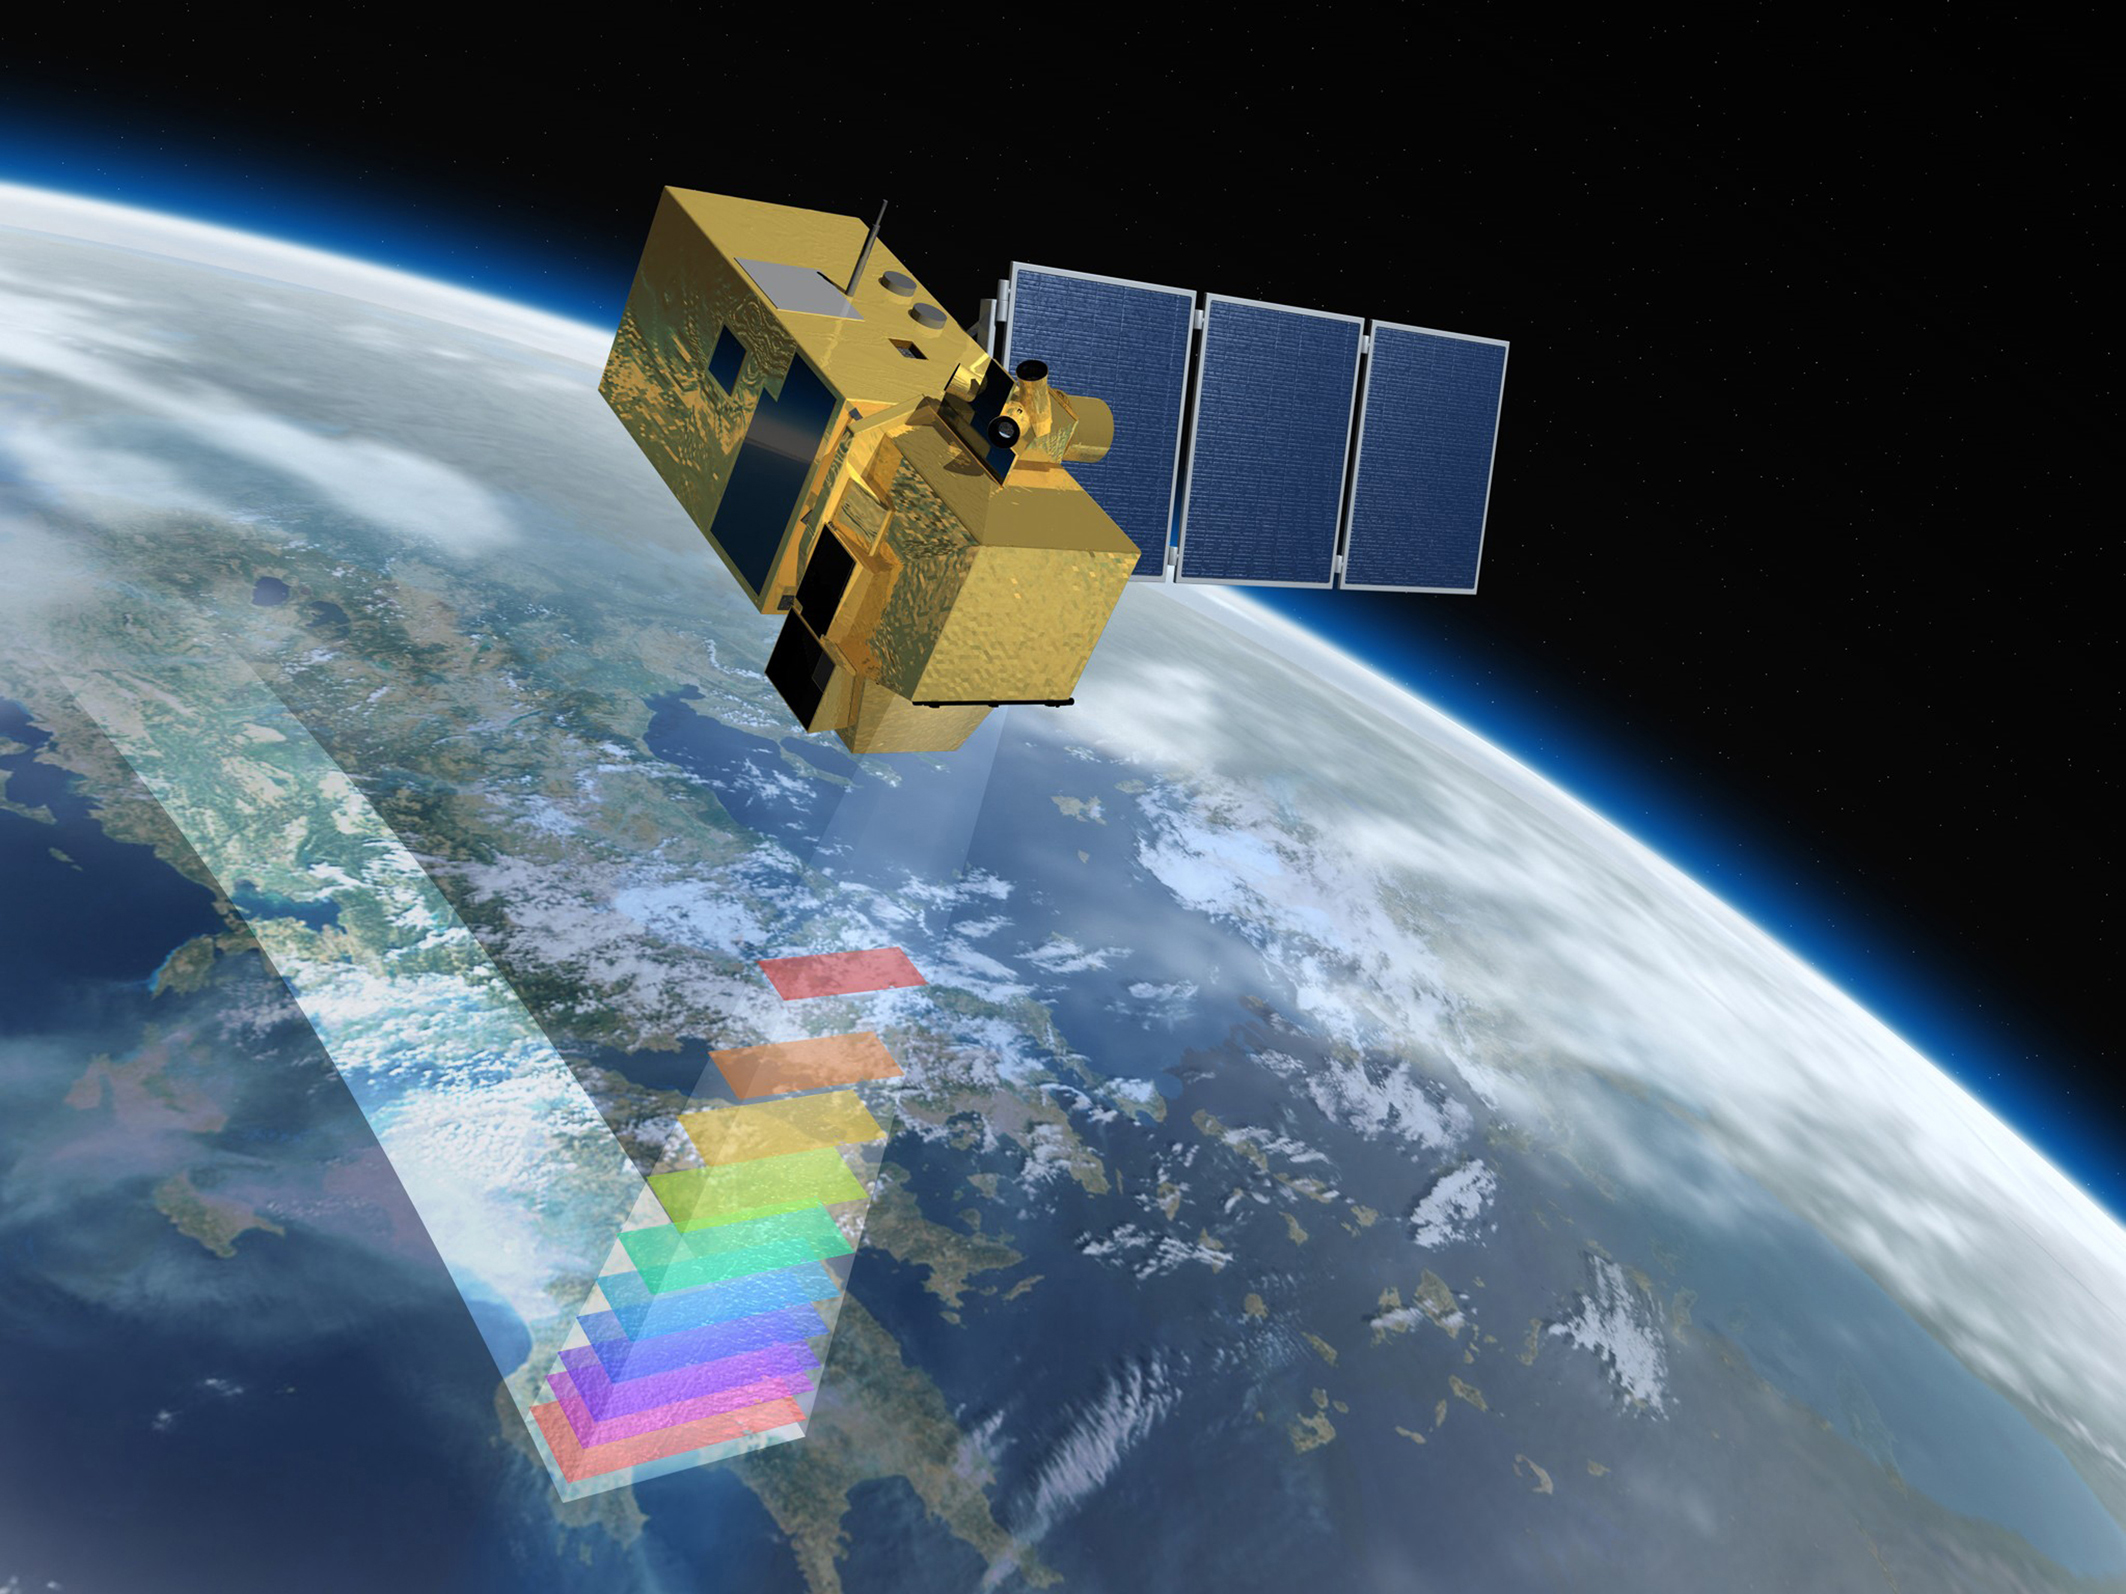
\includegraphics[width=15cm]{images/sentinel2}};
%	\node[below=of s2, text width=20cm]{
%	ESA Sentinel 2 Satellite
%	\begin{itemize}\setlength\itemsep{.1em}
%		\item 13 spectral bands
%		\item every 2-10 days
%		\item global coverage
%		\item free of charge	
%	\end{itemize}
%};
%\end{tikzpicture}
%}

%\newcommand{\modelbox}{
%	\begin{tikzpicture}[node distance=1em]
%\node(title){classification model $f$};
%\node[below=of title](large){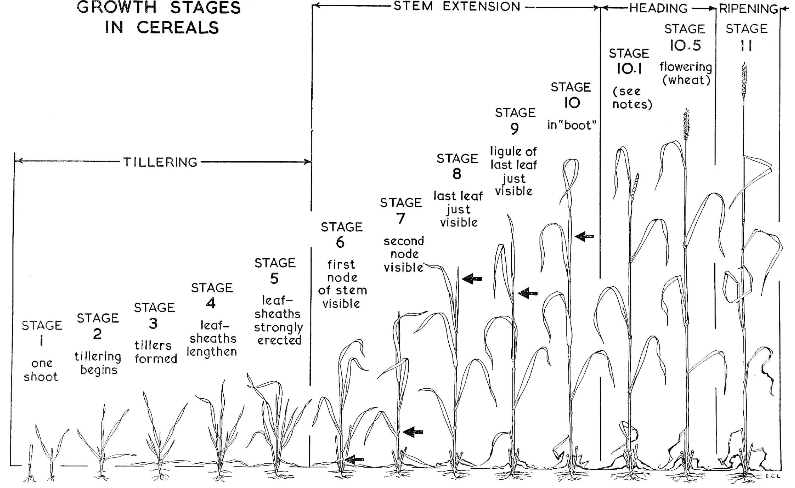
\includegraphics[width=15cm]{images/Large1954_cerial_growth_stages.png}};
%\node[below=of large](label){learning a phenological model};
%
%\node[below=3em of label, xshift=-5em, anchor=east]{yield};
%\node[below=3em of label, anchor=center]{health};
%\node[below=3em of label, xshift=5em, anchor=west]{droughts};
%
%
%\end{tikzpicture}
%}

%\newcommand{\labelbox}{
%\begin{tikzpicture}[node distance=1em]
%\node(title){crop type labels $\V{y}$};
%\node[below=of title](large){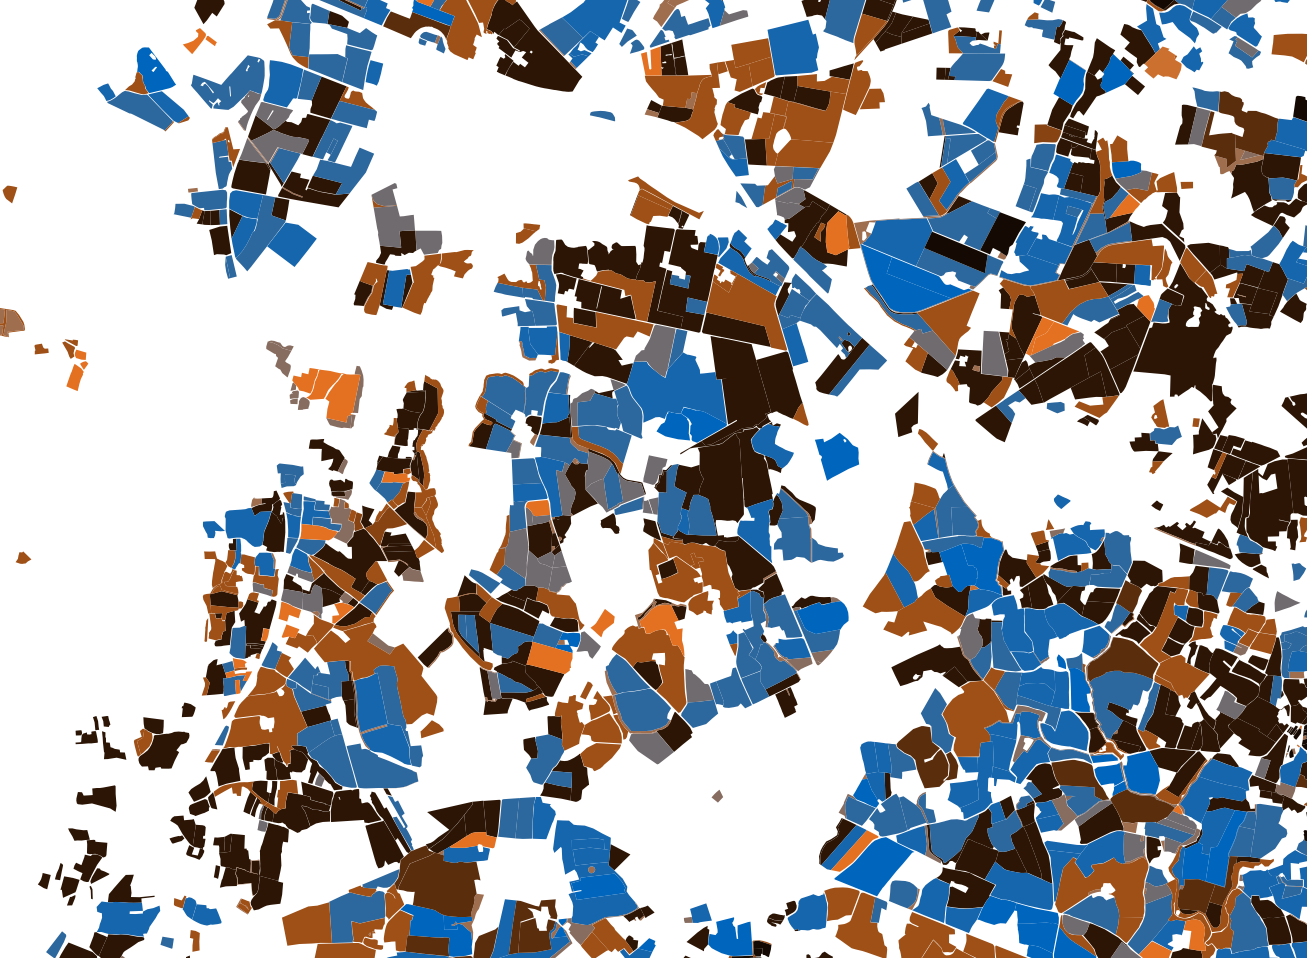
\includegraphics[width=15cm]{images/map/parcels}};
%\node[below=of large, text width=20cm]{
%Crop Type Labels
%\begin{itemize}\setlength\itemsep{.1em}
%\item Europes Common Agricultural Policy (CAP)
%\item reported by respective farmer
%\item gathered by national institutions (IGN in France)
%\end{itemize}
%};
%\end{tikzpicture}
%}

\begin{minipage}[t]{0.65\textwidth}

\section{The Objective}

\begin{tikzpicture}[scale=17]
	\node[label=Satellite Data ](x) at (-1,0){$\M{X} = (\V{x}_0, \V{x}_1, \dots , \V{x}_T)$};
	\node[below=of x, label=below:ESA Sentinel 2](s2){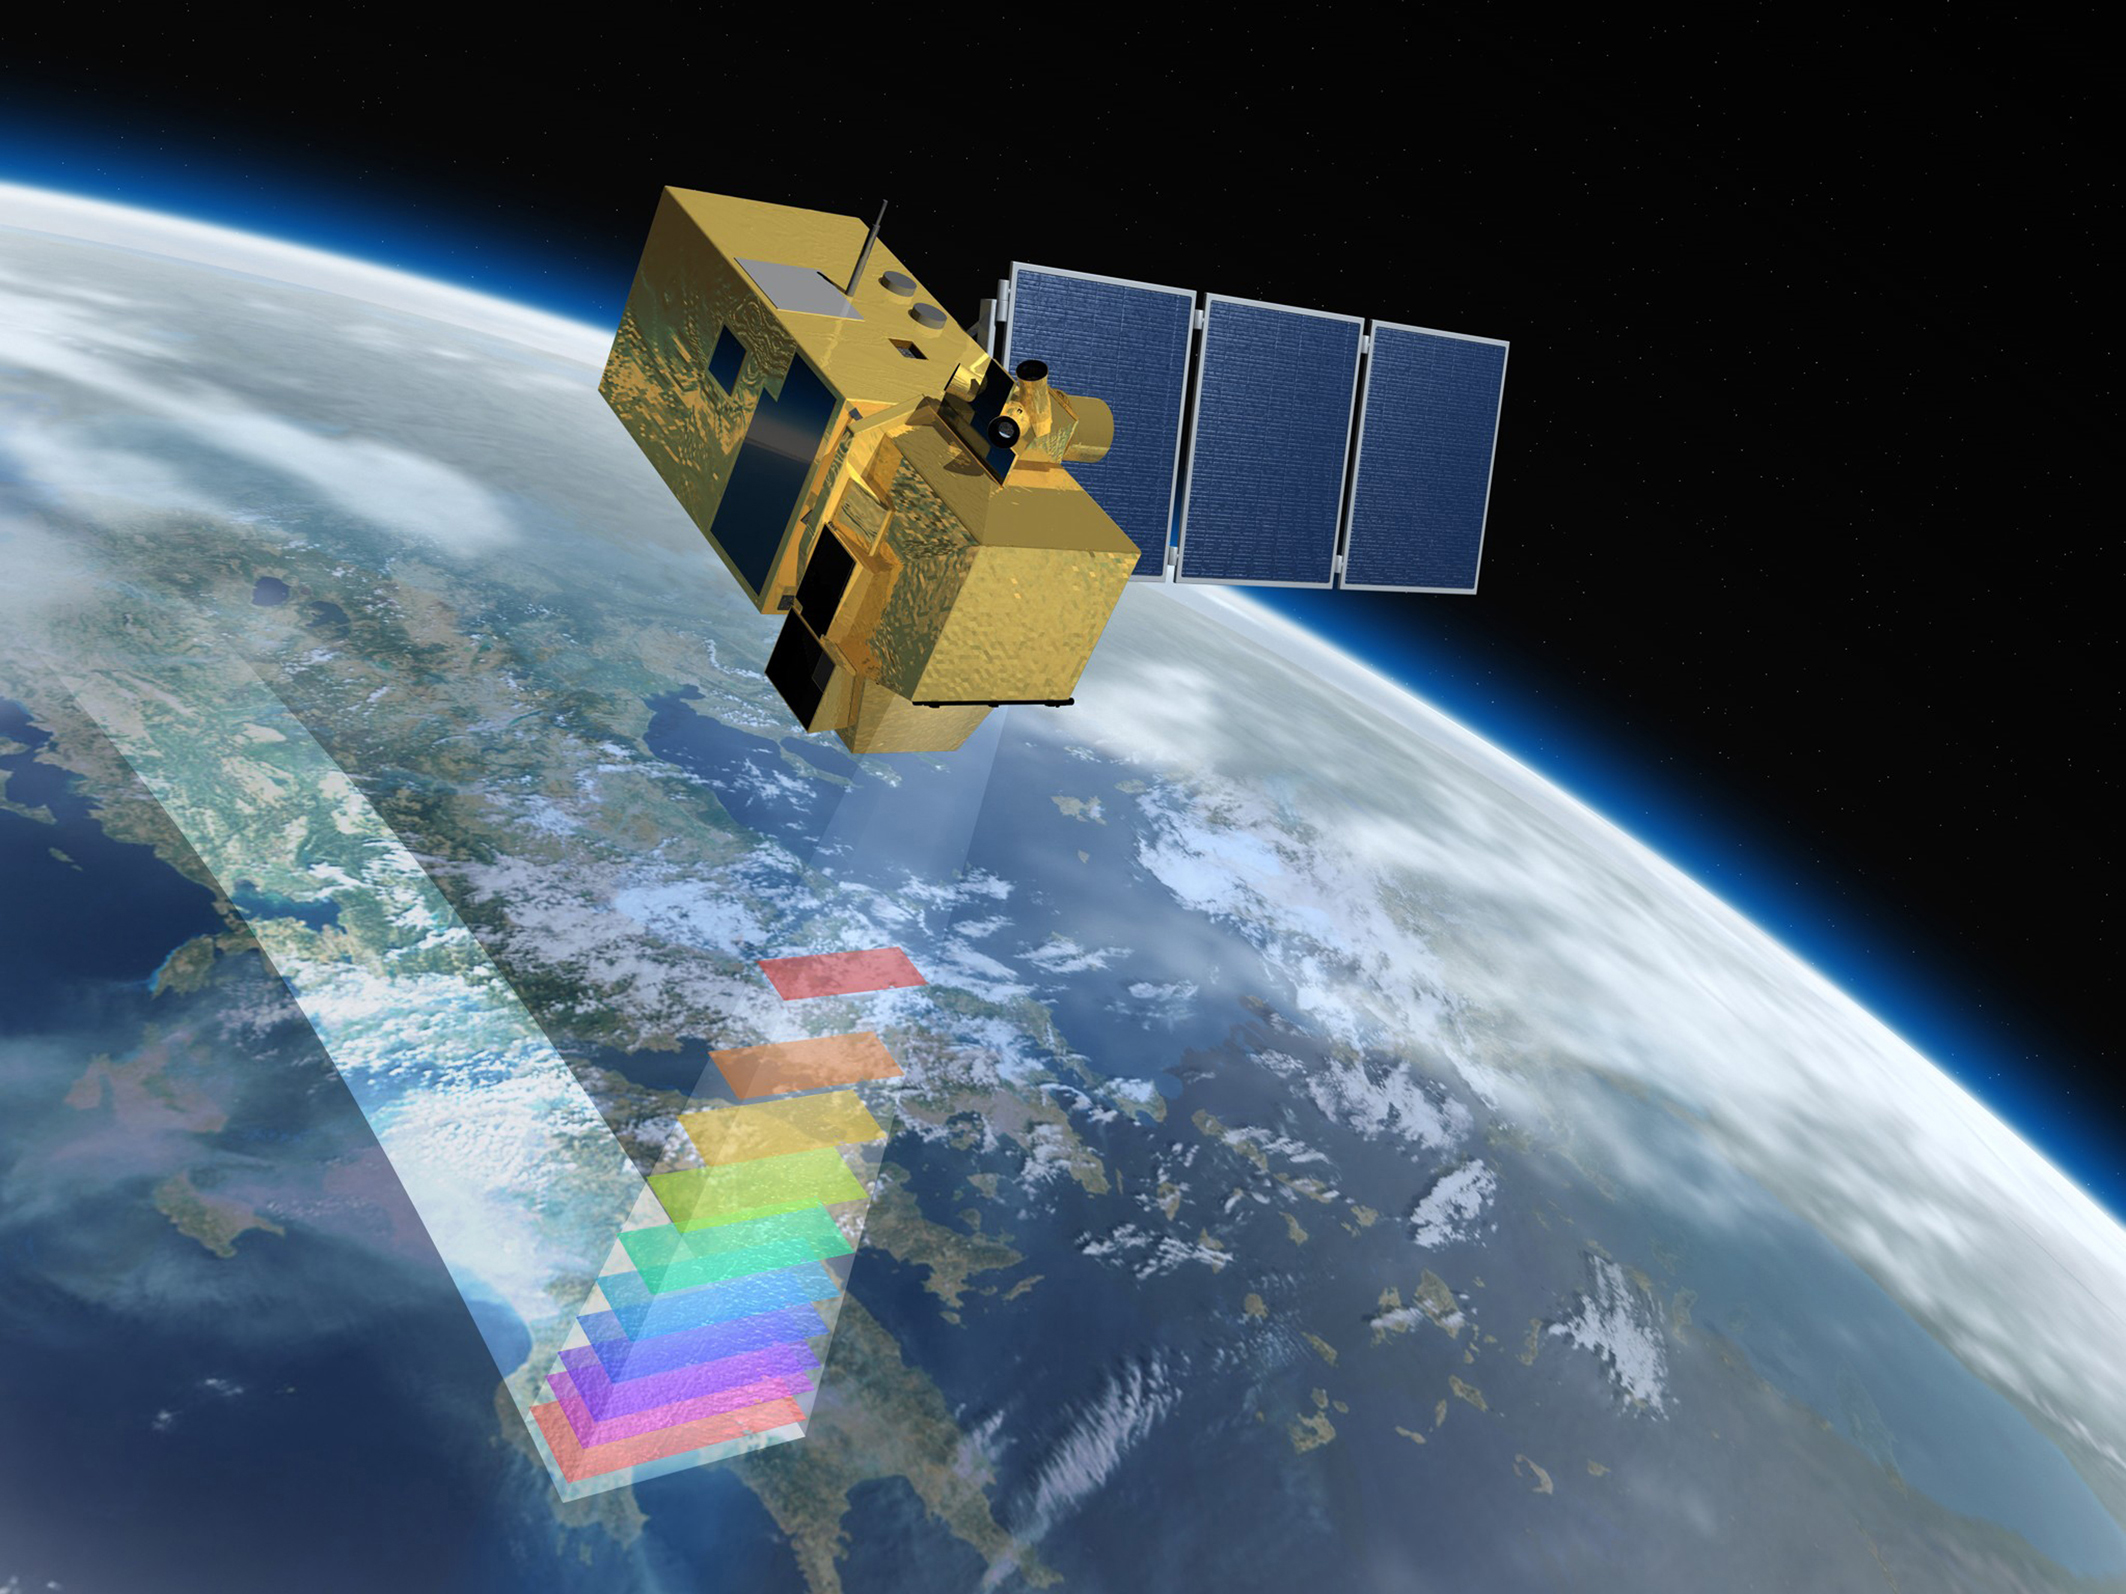
\includegraphics[width=13cm]{images/sentinel2}};
%	\node[below=of s2, text width=15cm]{
%		ESA Sentinel 2 Satellite
%		\begin{itemize}\setlength\itemsep{.1em}
%		\item 13 spectral bands
%		\item every 2-10 days
%		\item global coverage
%		\item free of charge	
%		\end{itemize}
%	};
	\node[below=of s2](eqbox){
		\begin{tikzpicture}[scale=4, anchor=center]
		
			\node at (1,0){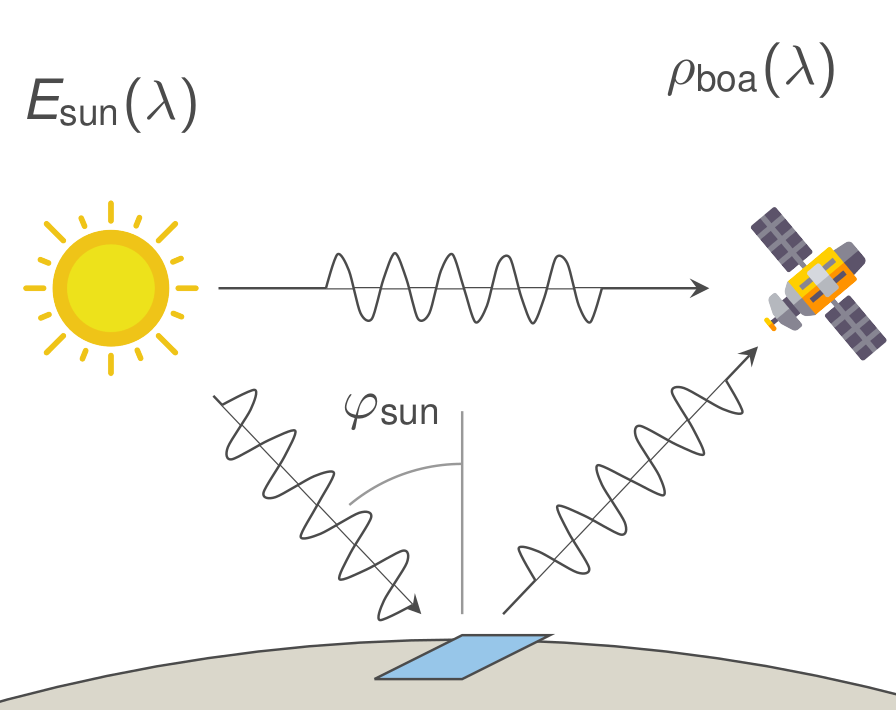
\includegraphics[width=8cm]{images/reflectance}};
			\node(eq) at (-1,0) {
				$
				\rho_\lambda = 
				\frac{
					\pi L_\lambda d^2
				}
				{
					E_\text{sun} \cos(\varphi_\text{sun})
				}
				$
				};
			\node at (0,-1){$\V{x}_t = \small \left(\rho_{\text{red}},\rho_{\text{green}},\rho_{\text{blue}},\rho_{\text{nir}},\dots\right)$};
		\end{tikzpicture}
	};
	
	\node[label=Classification Model](f) at (0,0){ $\V{y} = f(\V{x})$};
	\node[below=of f](large){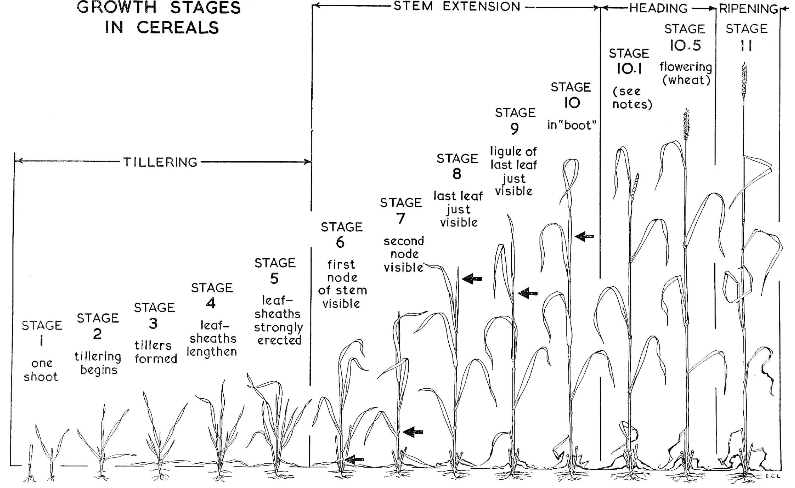
\includegraphics[width=13cm]{images/Large1954_cerial_growth_stages.png}};
	\node[below=of large, circle, fill=tumbluedark, text=white, text width=10cm](label){learning a \\ \textbf{\Large\color{tumorange}vegetation} \color{tumwhite} model};
	
	\node[label=Crop Type Labels ](y) at (1,0){$\V{y} \in \small \{\text{corn}, \text{meadows}, \dots\}$};
	\node[below=of y, label=below:IGN crop type labels](labels){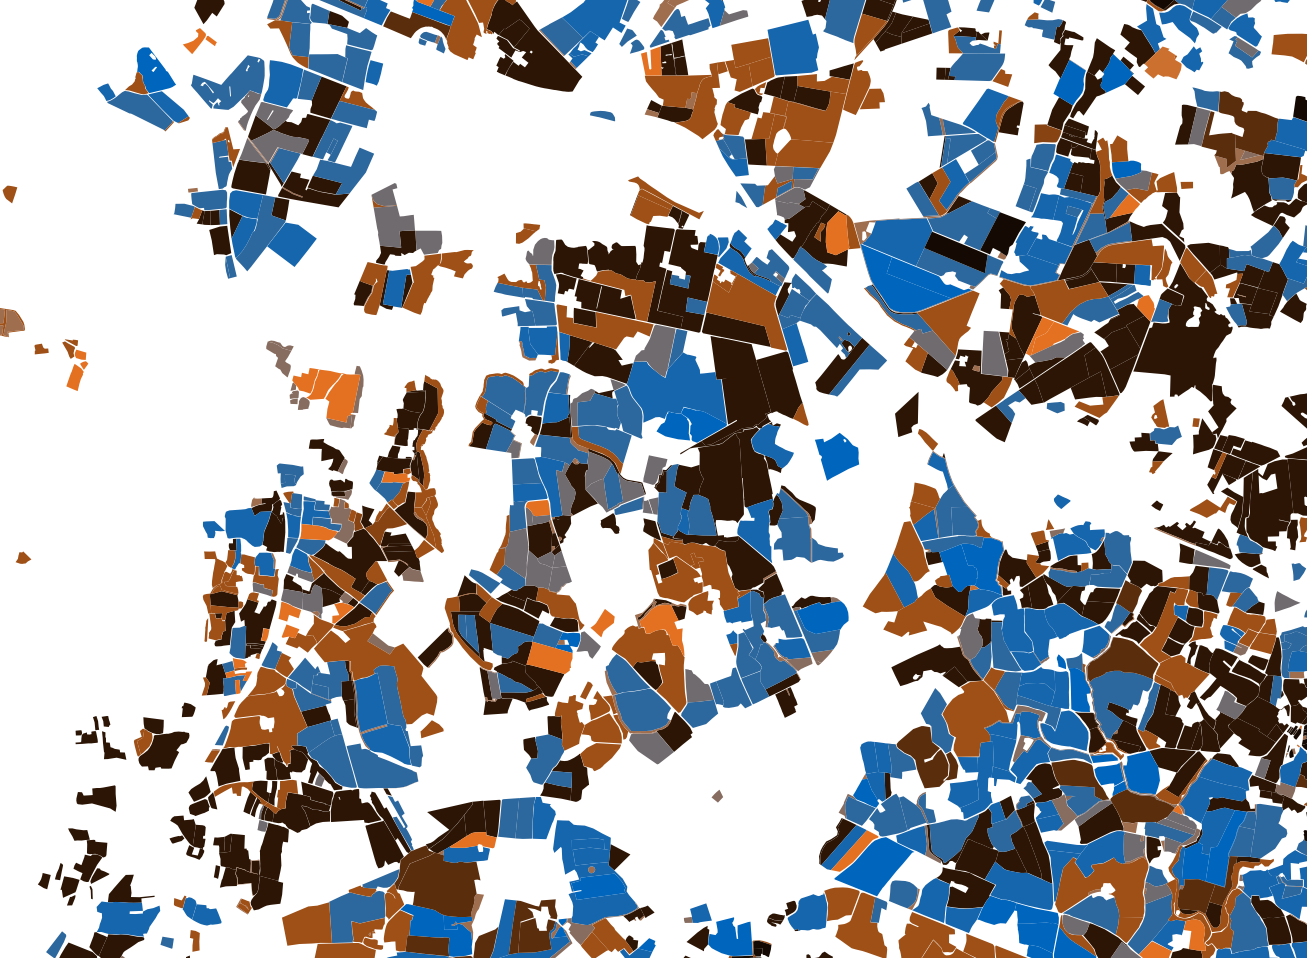
\includegraphics[width=13cm]{images/map/parcels}};
	\node[below=of labels, text width=12cm]{
		\small
	\begin{itemize}\setlength\itemsep{.1em}
		\item collected in entire Europe
		\item Europes Common Agricultural Policy (CAP)
		\item reported by respective farmer
		\item yearly data
		\item slowly made publicly available (INSPIRE)
	\end{itemize}
	};
	
	\draw (x) -- (f) -- (y);
\end{tikzpicture}

\section{Baselines}

\begin{tabular}{lrrrrrrr}
	\toprule
	baseline & accuracy & $\kappa$ & mean f1 & mean precision  & mean recall \\
	\cmidrule(lr){1-1}\cmidrule(lr){2-2}\cmidrule(lr){3-3}\cmidrule(lr){4-4}\cmidrule(lr){5-5}\cmidrule(lr){6-6}\cmidrule(lr){7-7}
	Transformer & \textbf{0.69}  &  \textbf{0.63} & 0.57 & {0.60} & 0.56 \\
	LSTM & 0.68 & 0.62 & \textbf{0.59} & \textbf{0.63} & \textbf{0.58} \\
	\bottomrule
\end{tabular}

\end{minipage}
\hfill
\begin{minipage}[t]{0.32\textwidth}
	
	\section{Challenges}
	
	This real-world dataset poses a series of Challenges to the Time Series Community
	
	\begin{itemize}
		\item agriculture dominated by some extensively cultivated crops
	\end{itemize}
%Agricultural areas are commonly dominated by few common crops, such as \textsl{corn}, \textsl{meadow}, or \textsl{wheat} which are cultivated This introduces a strong imbalance in the class frequencies, as shown in \cref{fig:classfrequencies}.
%	Please note the logarithmic scale. 
	
	\subsection{Similar Categories} 
%	\textbf{Classes with similar characteristics}
	\begin{itemize}
		\item some classes are vegetation-wise similar
	\end{itemize} 

	\tikzstyle{crop} = [fill=tumbluelight, rounded corners]
	
	\begin{tikzpicture}[xscale=13, yscale=5]
		\node at (0,0){{\verytiny\begin{tabular}{rlcccc}
\toprule
\textbf{\#} & \textbf{crop type} &  \textbf{prec.} & \textbf{rec.} & \textbf{$f_1$} & \textbf{\#samples} \\
\cmidrule(lr){1-1}\cmidrule(lr){2-2}\cmidrule(lr){3-3}\cmidrule(lr){4-4}\cmidrule(lr){5-5}\cmidrule(lr){6-6}
%\midrule
1 & barley &         90 &          86 &          88 &     4982 \\
2 & wheat &         83 &          95 &          89 &    13850 \\
3 & corn &         93 &          \textbf{96} &          94 &    25059 \\
4 & fodder &         51 &          34 &          41 &     3449 \\
5 & fallow &         30 &           2 &           4 &     3863 \\
6 & misc. &         50 &          49 &          49 &    12499 \\
7 & orchards &         21 &           7 &          10 &      391 \\
8 & cereals &         74 &          47 &          57 &     4645 \\
9 & perm. meadows &         51 &          47 &          49 &    20966 \\
10 & protein crops &         42 &          61 &          50 &      498 \\
11 & rapeseed &         \textbf{96} &          94 &          \textbf{95} &     2664 \\
12 & temp. meadows &         56 &          68 &          62 &    29977 \\
13 & vegetables &         86 &          69 &          76 &     3114 \\
   &                       &            &             &             &          \\
   &                       &         \textbf{63} &          \textbf{58} &          \textbf{59} &   125957 \\
\bottomrule
\end{tabular}

}};
		\node at (1,0){\resizebox{10cm}{!}{\confmat{images/data/BreizhCrops_rnn/npy/confmat_flat.csv}{3}{1}}};
%		\node at (1,-1){\resizebox{10cm}{!}{\confmat{images/data/BreizhCrops_rnn/npy/confmat_flat.csv}{3}{1}}};
	\end{tikzpicture}




	
	

%Some categories can be traced to one unique type of crop, such as \textsl{wheat}, or \textsl{corn}. 
%	Here, the phenological characteristics can be traced to single specific crop types.
%	Other, less frequent classes, are aggregated into groups that incorporate a broader range of vegetation types which may be difficult to distinguish, such as \emph{orchards}.
%	
	\subsection{Clouds introduce noise}

	\begin{tikzpicture}
		\tikzsetnextfilename{example}

\newcommand{\example}[1]{
	
\begin{tikzpicture}
	
	\tikzstyle{annot} = [font=\tiny\sffamily, text=tumblue]
	\tikzstyle{point} = [thin, tumbluelight, shorten >= .25em, shorten <= .25em]
	
	% from /home/marc/projects/EV2019/images/example/tstop.txt
	\def\tstopv{0.6285714285714286}
	\def\class{winter barley}
	
	\begin{axis}[date coordinates in=x,
	date ZERO=2017-01-01,
	xmin=2017-01-01,
	xmax=2017-12-31,
	ylabel near ticks,
	ylabel style={font=\sffamily\small, rotate=0},
	width=\textwidth,
	height=7cm,
	axis x line=bottom,
	axis y line=left,
	%	enlarge x limits=0.01,
	xtick={2017-01-01,2017-05-01,2017-08-01,2017-12-01},
	xticklabels={January,April,August,December},
	ymajorgrids,
	ymax=10000,
	very thin,
	smooth,
	no marks,  
	ylabel={$\rho \times 10^4$},
	draw opacity=.8,
	%		tension=0.001,
	legend columns=2,
	%y tick label style={rotate=90},
	legend style={at={(.5,1)},anchor=south, line width=1pt, fill=tumblue!10}
	]
	
	
	\addplot[b1color] table [x=doa, y=B1, col sep=comma, forget plot] {#1};
	\addplot[b9color] table [x=doa, y=B9, col sep=comma, forget plot] {#1};
	\addplot[b10color] table [x=doa, y=B10, col sep=comma] {#1};
	
	\addplot[b11color] table [x=doa, y=B11, col sep=comma, forget plot] {#1};
	\addplot[b12color] table [x=doa, y=B12, col sep=comma] {#1};
	
	\addplot[b5color] table [x=doa, y=B5, col sep=comma, forget plot] {#1};
	\addplot[b6color] table [x=doa, y=B6, col sep=comma, forget plot] {#1};
	\addplot[b7color] table [x=doa, y=B7, col sep=comma, forget plot] {#1};
	\addplot[b8color] table [x=doa, y=B8, col sep=comma, forget plot] {#1};
	\addplot[b8Acolor] table [x=doa, y=B8A, col sep=comma] {#1};
	
	\addplot[b2color] table [x=doa, y=B2, col sep=comma, forget plot] {#1};
	\addplot[b3color] table [x=doa, y=B3, col sep=comma, forget plot] {#1};
	\addplot[b4color] table [x=doa, y=B4, col sep=comma] {#1};
	
	
	\legend{3 atmospheric, 2 short-wave infrared, 5 near infrared, 3 visible bands}
	
	\end{axis}

	\end{tikzpicture}
	
}

%\newcommand{\wv}[2]{$\lambda_\text{#1}=#2$}
\newcommand{\wv}[2]{$\rho_{\lambda=\text{#2}}$}


\newcommand{\examplemeadows}{

\begin{tikzpicture}


\tikzstyle{annot} = [font=\tiny\sffamily, text=tumblue]
\tikzstyle{point} = [thin, tumbluelight, shorten >= .25em, shorten <= .25em]

% from /home/marc/projects/EV2019/images/example/tstop.txt
\def\tstopv{0.6285714285714286}
\def\class{winter barley}

\begin{axis}[date coordinates in=x,
date ZERO=2017-01-01,
xmin=2017-01-01,
xmax=2017-12-31,
ylabel near ticks,
ylabel style={font=\sffamily\small, rotate=0, yshift=-.5em},
width=20cm,
height=5cm,
axis x line=bottom,
axis y line=left,
%	enlarge x limits=0.01,
xtick={2017-01-01,2017-05-01,2017-08-01,2017-12-01},
xticklabels={January,April,August,December},
ymajorgrids,
ymax=10000,
thin,
smooth,
no marks,  
ylabel={$\rho \times 10^4$},
draw opacity=.8,
%		tension=0.001,
legend columns=13,
%y tick label style={rotate=90},
%legend to name=leg,
legend style={at={(-.3,-.7		)},anchor=north, line width=1pt, name=legend, fill=tumblue!10,font=\scriptsize\sffamily},
legend image post style={line width =4pt}
]

%\addlegendimage{empty legend}


\addplot[b1color] table [x=doa, y=B1, col sep=comma] {images/example/3685593.csv};
\addplot[b2color] table [x=doa, y=B2, col sep=comma] {images/example/3685593.csv};
\addplot[b3color] table [x=doa, y=B3, col sep=comma] {images/example/3685593.csv};
\addplot[b4color] table [x=doa, y=B4, col sep=comma] {images/example/3685593.csv};
\addplot[b5color] table [x=doa, y=B5, col sep=comma] {images/example/3685593.csv};
\addplot[b6color] table [x=doa, y=B6, col sep=comma] {images/example/3685593.csv};
\addplot[b7color] table [x=doa, y=B7, col sep=comma] {images/example/3685593.csv};
\addplot[b8color] table [x=doa, y=B8, col sep=comma] {images/example/3685593.csv};
\addplot[b8Acolor] table [x=doa, y=B8A, col sep=comma] {images/example/3685593.csv};
\addplot[b9color] table [x=doa, y=B9, col sep=comma] {images/example/3685593.csv};
\addplot[b10color] table [x=doa, y=B10, col sep=comma] {images/example/3685593.csv};
\addplot[b11color] table [x=doa, y=B11, col sep=comma] {images/example/3685593.csv};
\addplot[b12color] table [x=doa, y=B12, col sep=comma] {images/example/3685593.csv};

%\node[above=of leg]{test};
%
%\addlegendentry{$\sqrt{x}$}
%\addlegendentry{$\ln{x}$}
%
%\addlegendentry[xshift=-10pt, font=\bfseries]{S2 Satellite Bands}

%\addlegendentry{\wv{B01}{443nm}}
%\addlegendentry{\wv{B2}{492nm}}
%\addlegendentry{\wv{B3}{560nm}}
%\addlegendentry{\wv{B4}{665nm}}
%\addlegendentry{\wv{B5}{704nm}}
%\addlegendentry{\wv{B6}{740nm}}
%\addlegendentry{\wv{B7}{783nm}}
%\addlegendentry{\wv{B8}{833nm}}
%\addlegendentry{\wv{B8A}{864nm}}
%\addlegendentry{\wv{B9}{945nm}}
%\addlegendentry{\wv{B10}{1374nm}}
%\addlegendentry{\wv{B12}{2202nm}}

%\legend{
%\wv{B01}{443nm},
%\wv{B2}{492nm},
%\wv{B3}{560nm},
%\wv{B4}{665nm},
%\wv{B5}{704nm},
%\wv{B6}{740nm},
%\wv{B7}{783nm},
%\wv{B8}{833nm},
%\wv{B8A}{864nm},
%\wv{B9}{945nm},
%\wv{B10}{1374nm},
%\wv{B11}{1613nm},
%\wv{B12}{2202nm}}


\end{axis}

%\node[left=of legend, font=\scriptsize\sffamily]{Sentinel 2 Satellite Spectral Bands};
%\node[ anchor=west] at (0.2,2.7) {};


\end{tikzpicture}
}


\newcommand{\examplecorn}{
	
	\begin{tikzpicture}
	
	\tikzstyle{annot} = [font=\tiny\sffamily, text=tumblue]
	\tikzstyle{point} = [thin, tumbluelight, shorten >= .25em, shorten <= .25em]
	
	% from /home/marc/projects/EV2019/images/example/tstop.txt
	\def\tstopv{0.6285714285714286}
	\def\class{winter barley}
	
	\begin{axis}[date coordinates in=x,
	date ZERO=2017-01-01,
	xmin=2017-01-01,
	xmax=2017-12-31,
	ylabel near ticks,
	ylabel style={font=\sffamily\small, rotate=0, yshift=-.5em},
	width=20cm,
	height=5cm,
	axis x line=bottom,
	axis y line=left,
	%	enlarge x limits=0.01,
	xtick={2017-01-01,2017-05-01,2017-08-01,2017-12-01},
	xticklabels={January,April,August,December},
	ymajorgrids,
	ymax=10000,
	thin,
	smooth,
	no marks,  
	ylabel={$\rho \times 10^4$},
	draw opacity=.8,
	%		tension=0.001,
	legend columns=2,
	%y tick label style={rotate=90},
	legend style={at={(-.3,1.1)},anchor=south, line width=1pt, fill=tumblue!10, font=\small}
	]
	
	
	\addplot[b1color] table [x=doa, y=B1, col sep=comma] {images/example/6139251.csv};
	\addplot[b9color] table [x=doa, y=B9, col sep=comma] {images/example/6139251.csv};
	\addplot[b10color] table [x=doa, y=B10, col sep=comma] {images/example/6139251.csv};
	
	\addplot[b11color] table [x=doa, y=B11, col sep=comma] {images/example/6139251.csv};
	\addplot[b12color] table [x=doa, y=B12, col sep=comma] {images/example/6139251.csv};
	
	\addplot[b5color] table [x=doa, y=B5, col sep=comma] {images/example/6139251.csv};
	\addplot[b6color] table [x=doa, y=B6, col sep=comma] {images/example/6139251.csv};
	\addplot[b7color] table [x=doa, y=B7, col sep=comma] {images/example/6139251.csv};
	\addplot[b8color] table [x=doa, y=B8, col sep=comma] {images/example/6139251.csv};
	\addplot[b8Acolor] table [x=doa, y=B8A, col sep=comma] {images/example/6139251.csv};
	
	\addplot[b2color] table [x=doa, y=B2, col sep=comma] {images/example/6139251.csv};
	\addplot[b3color] table [x=doa, y=B3, col sep=comma] {images/example/6139251.csv};
	\addplot[b4color] table [x=doa, y=B4, col sep=comma] {images/example/6139251.csv};
	
	\node[font=\sffamily\tiny, text=tumblue] at (rel axis cs:0.25,0.90)(gr){ground signal};
	\draw[draw=tumblue] (gr) -- (rel axis cs:.26,.3);
	\draw[draw=tumblue] (gr) -- (rel axis cs:.2,.3);
	\draw[draw=tumblue] (gr) -- (rel axis cs:.4,.25);
	
	\node[font=\sffamily\tiny, text=tumblue] at (rel axis cs:0.85,.93)(cl){cloud noise};
	
	\draw[draw=tumblue] (cl) -- (rel axis cs:.68,.7);
	\draw[draw=tumblue] (cl) -- (rel axis cs:.58,.7);
	\draw[draw=tumblue] (cl) -- (rel axis cs:.81,.7);
	
%	\legend{3 atmospheric, 2 short-wave infrared, 5 near infrared, 3 visible bands}
%	
	\end{axis}
	
	\end{tikzpicture}
}
		\node at (0,0){\examplecorn};
	\end{tikzpicture}
%	\textbf{Non-Gaussian noise induced by clouds}. Clouds cover the Earth's surface at regular intervals. Their large reflectance introduces a positive non-gaussian noise to the data at single intervals. 
%	This manifests itself by positive outliers in the reflectance data over the time scale, as can be seen in the examples of \cref{fig:aoi}.
%	

	\textbf{Regional Variations in class distributions and imbalanced class labels}
%	\textbf{Regional variations in the class distributions}. Regional variances in soil quality, elevation, temperature, and precipitation lead to a spatial correlation in the frequency of dominated agricultural crop. This effect increases at larger scales where these environmental conditions change significantly.
%	Still, certain variations in crop distributions based on regionally distinct regions can be seen in \cref{fig:classfrequencies}.
	
	\tikzsetnextfilename{partition_histograms}
\begin{tikzpicture}
  \begin{axis}[
        ybar, 
        axis on top,
        title={},
        height=8cm, width=.66\textwidth,
        bar width=.1em,
        ymajorgrids, 
        tick align=outside,
%        major grid style={draw=tumwhite},
%        enlarge y limits={value=.1,upper},
        ymin=0,
%        axis x line*=bottom,
%        axis y line*=left,
        ymode=log,
        axis line style={opacity=1, thin},
%        tickwidth=1pt,
        enlarge x limits=.05,
%        legend style={
%            at={(0.6,1.2)},
%            anchor=south,
%            draw=none,
%            legend columns=1,
%            rounded corners=0,
%            /tikz/every even column/.append style={column sep=0.5cm, font=\scriptsize}
%        },
        ylabel={Number of Parcels},
        ylabel style={yshift=1.3em},
%        xlabel style={yshift=2em},
%        x tick label style={yshift=-1em},
        xtick={0,1,...,12},
        xticklabels={\tiny barley, wheat, corn, fodder, fallow, misc., orchards, cereals, perm. meadows, protein crops, rapeseed, temp. meadows, vegetables},
        tick label style={rotate=20,anchor=east}
%        x tick label style={align=right,text width=3.5cm},
%       xticklabel style = {rotate=90,anchor=east},
       %nodes near coords={
       % \tiny \pgfmathprintnumber[precision=0]{\pgfplotspointmeta}
       %}
    ]
    \addplot [draw=none, fill=frh01color] table[x=id,y=frh01, col sep=comma] {images/counts.csv};
    \addplot [draw=none, fill=frh02color] table[x=id,y=frh02, col sep=comma] {images/counts.csv};
    \addplot [draw=none, fill=frh03color] table[x=id,y=frh03, col sep=comma] {images/counts.csv};
    \addplot [draw=none, fill=frh04color] table[x=id,y=frh04, col sep=comma] {images/counts.csv};

%    \legend{Côtes-d’Armor {\tiny(FRH01)},Finistère {\tiny(FRH02)},Ille-et-Vilaine {\tiny(FRH03)},Morbihan {\tiny(FRH04)}}
  \end{axis}
  
  \node at (20,2){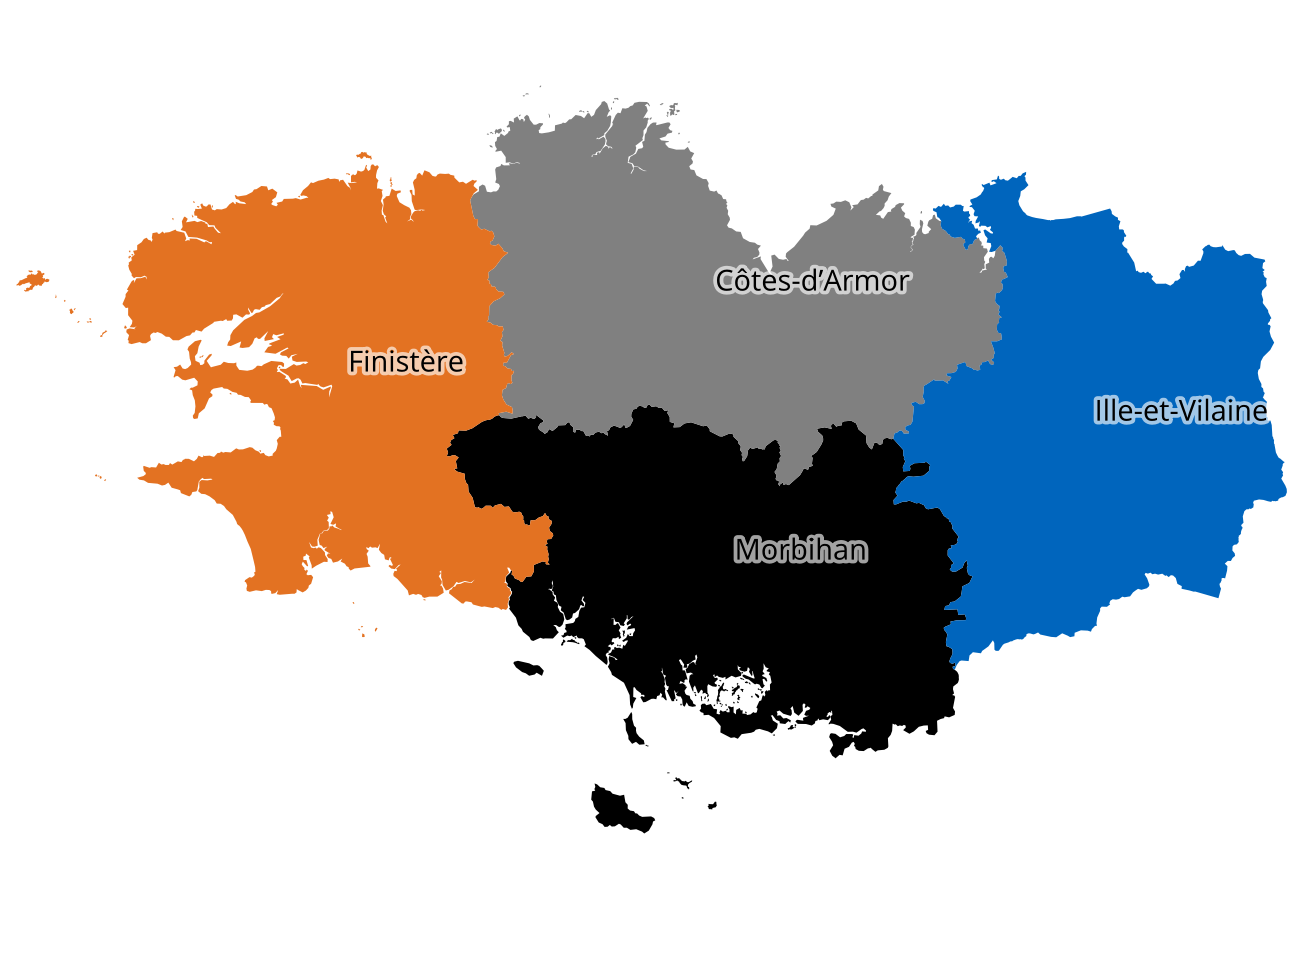
\includegraphics[width=8cm]{images/map/regions}};
  \end{tikzpicture}
	
%	
%	\begin{tikzpicture}
%		\node at (0,1){
%			
%		};
%	\end{tikzpicture}
%	
%	\begin{tikzpicture}
%
%\node at (1,-1){};
%	\end{tikzpicture}
%	
	\subsection{Irregular Sampling Distance and cariable sequence length}
	
	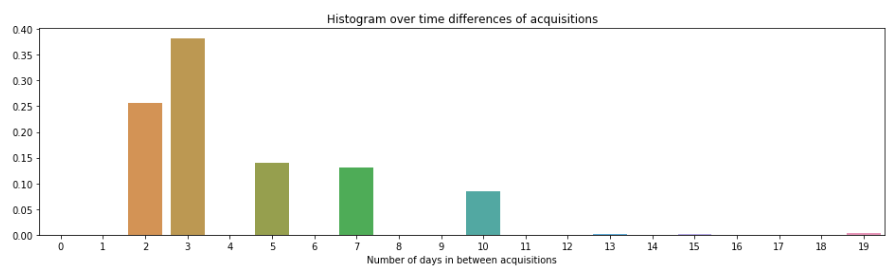
\includegraphics[width=\textwidth, height=3cm]{images/days_between_acquisitions}
	
	\subsection{Spatial Autocorrelation}
	 
	 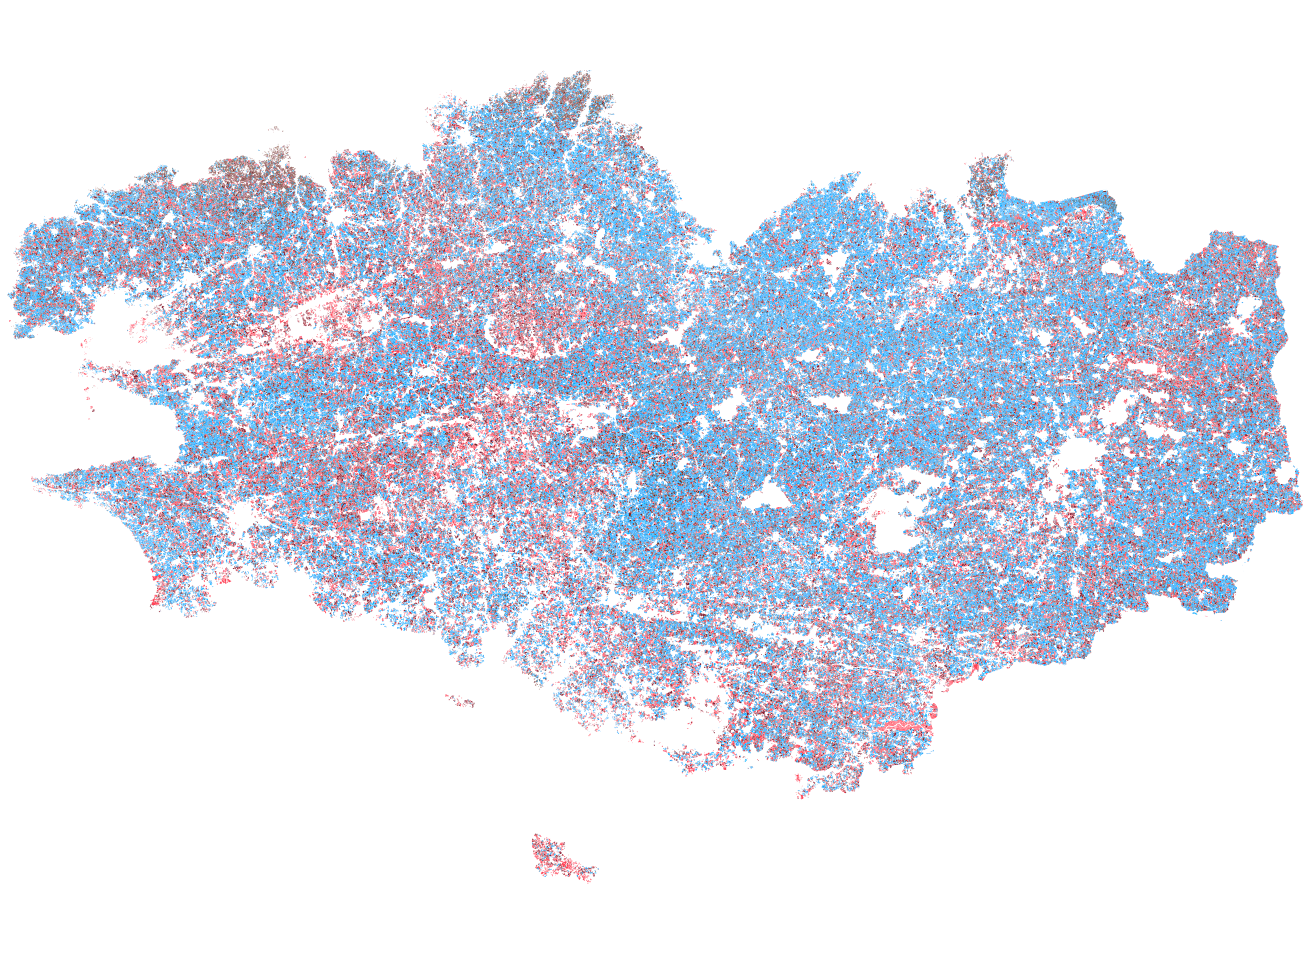
\includegraphics[width=.66\textwidth]{images/map/breizh}
	 
%	\textbf{Spatial autocorrelation}. Spatially closer objects are more similar than distant ones \citep{tobler1970computer}. This autocorrelation can introduce a dependence between training and validation datasets that may disguise overfitting and impede generalization. 
%	To counteract this, several researchers \cite{russwurm2017temporal,jean2018tile2vec} have adopted a training/validation/evaluation partitioning that groups spatially distant parcels.
%	%We encourage training on distinct regions in the dataset to ensure that training and test datasets are fully independent.
%	Hence, we organized the data in their respective NUTS-3 regions to encourage training on these spatially separate regions.
	
%	
%	\begin{tikzpicture}[scale=20]
%	\node[label=Satellite Data ](x) at (-1,0){$\M{X} = (\V{x}_0, \V{x}_1, \dots , \V{x}_T)$};
%	\node[below=of x, label=below:ESA Sentinel 2](s2){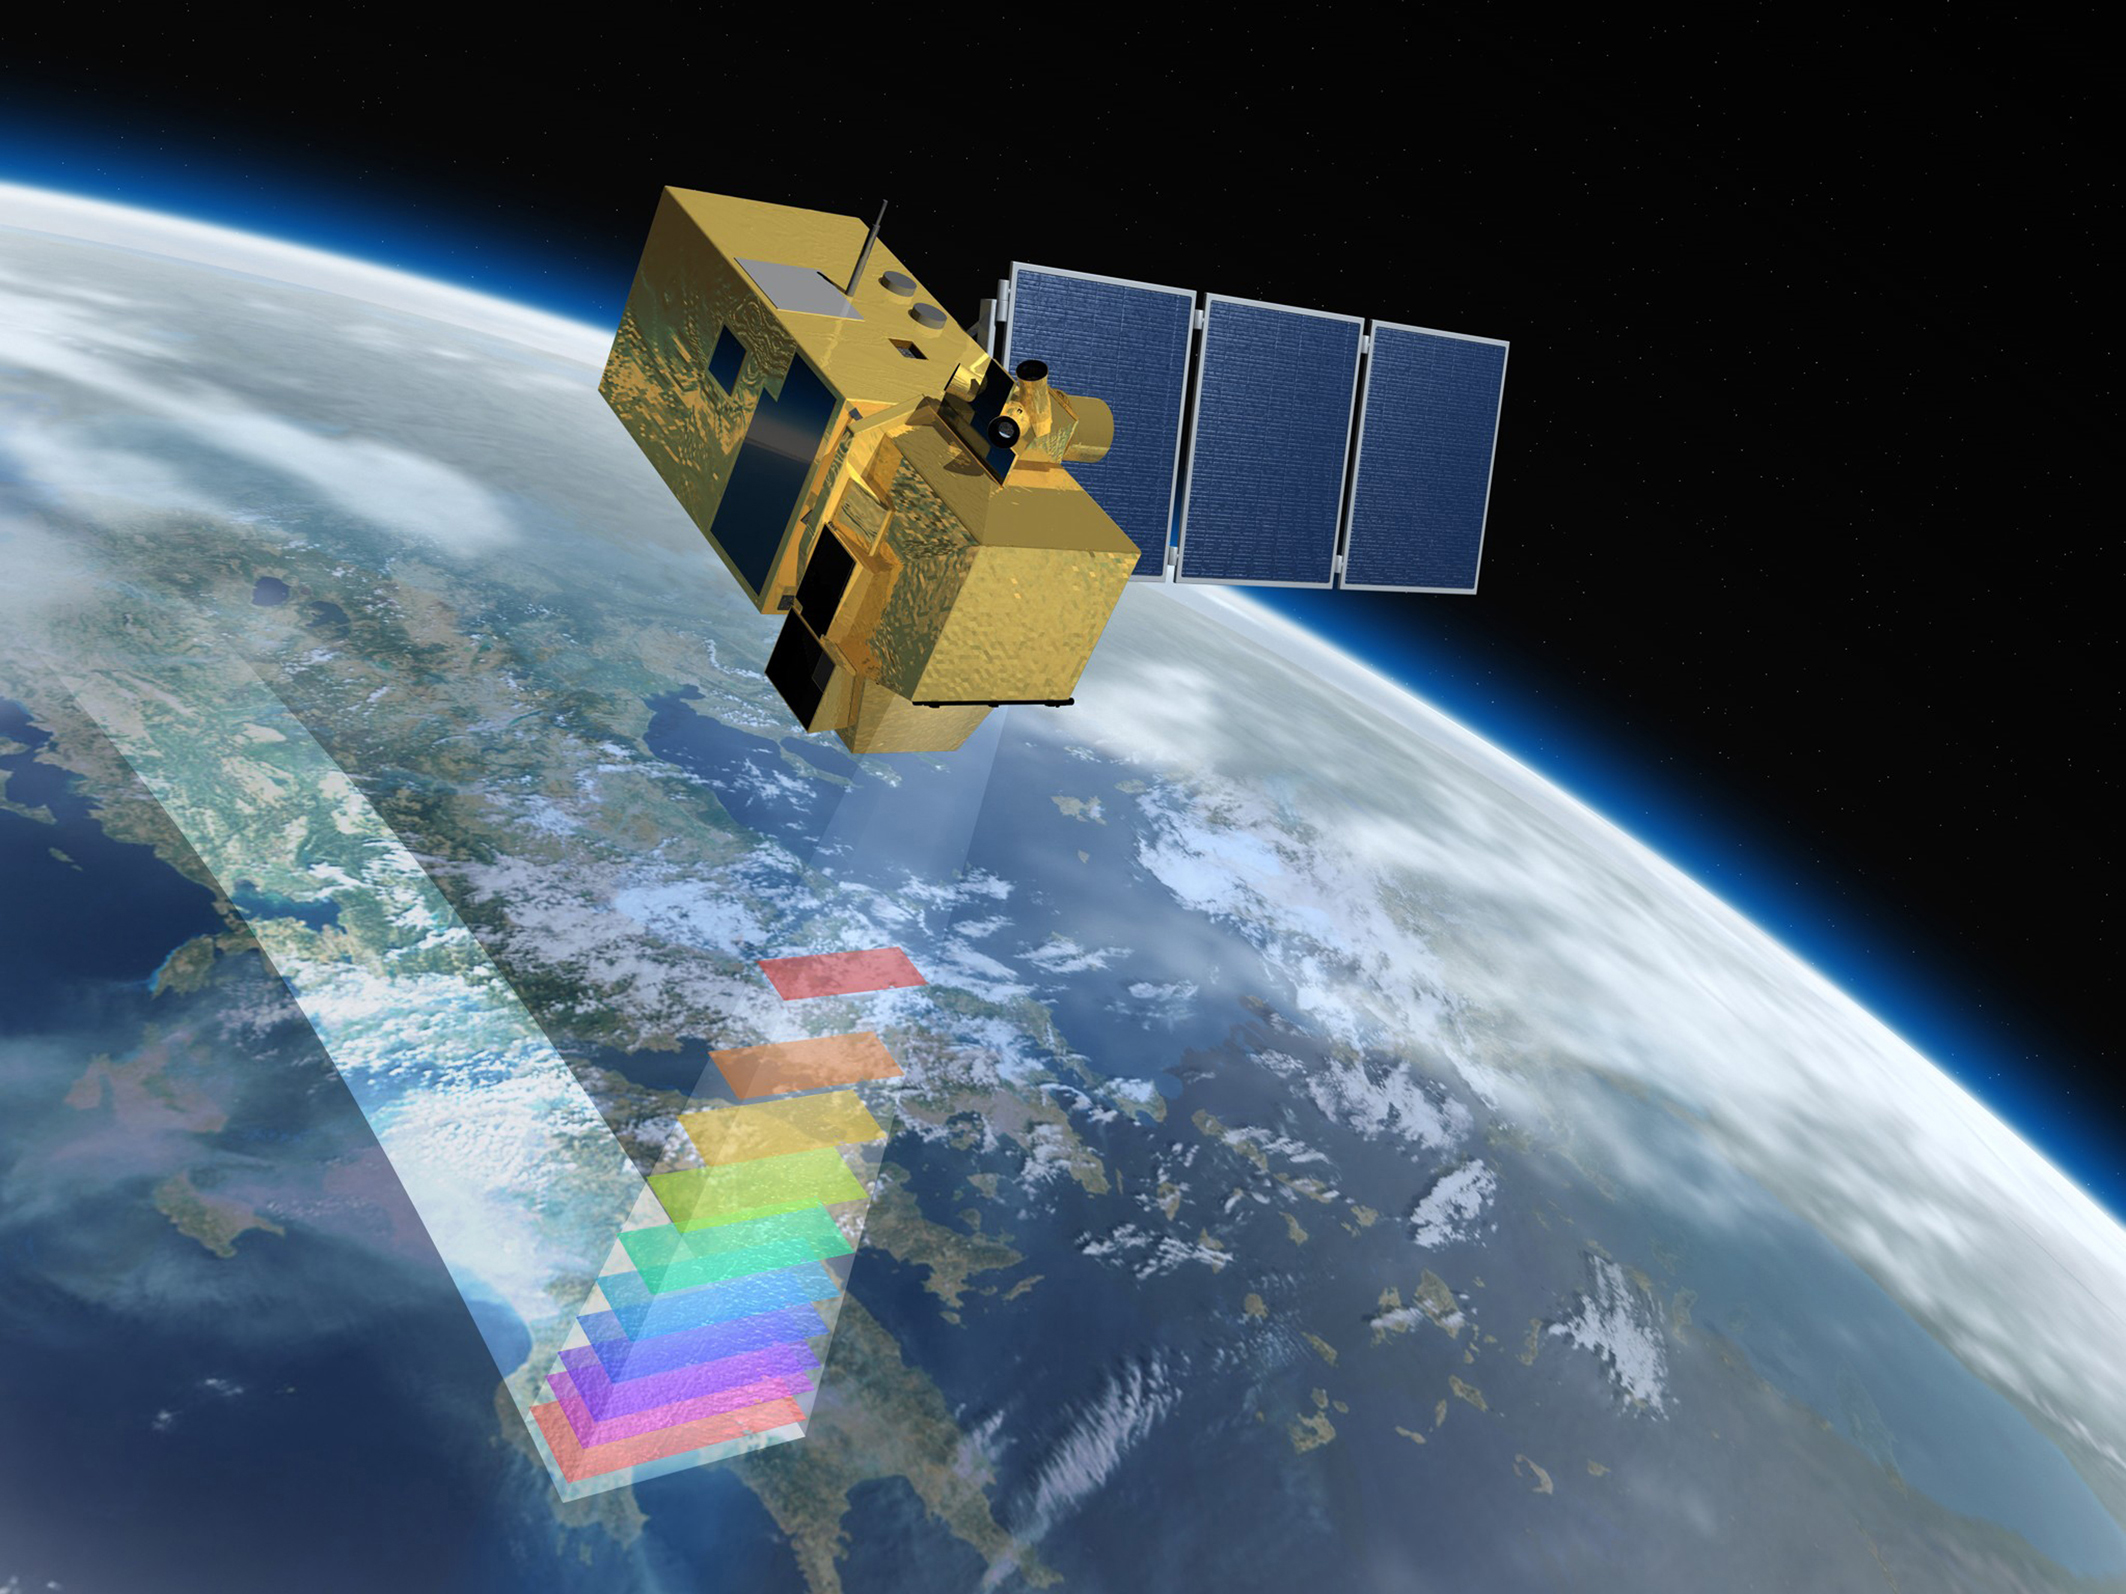
\includegraphics[width=15cm]{images/sentinel2}};
%	\node[below=of s2, text width=15cm]{
%		ESA Sentinel 2 Satellite
%		\begin{itemize}\setlength\itemsep{.1em}
%		\item 13 spectral bands
%		\item every 2-10 days
%		\item global coverage
%		\item free of charge	
%		\end{itemize}
%	};
%	
%	\node[label=classificaiton model](f) at (0,0){ $\V{y} = f(\V{x})$};
%	\node[below=of f](large){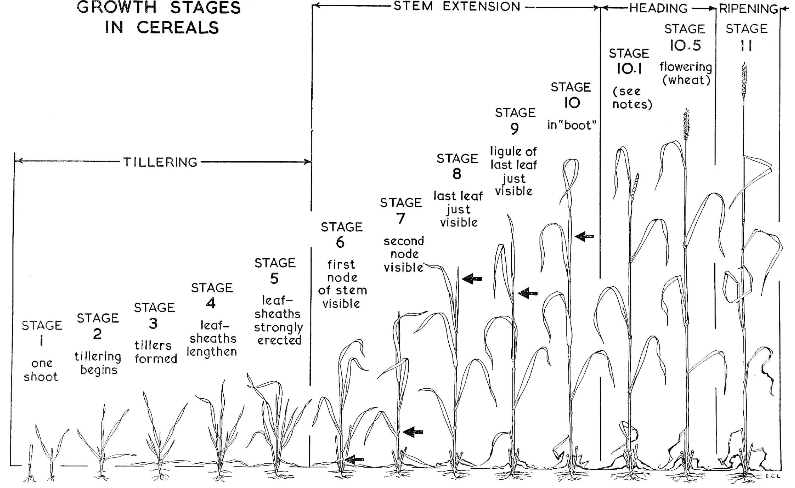
\includegraphics[width=15cm]{images/Large1954_cerial_growth_stages.png}};
%	\node[below=of large](label){Objective: learning a \textbf{vegetation model} $f$};
%	
%	\node[label=crop type labels ](y) at (1,0){$\V{y} \in \small \{\text{corn}, \text{meadows}, \dots\}$};
%	\node[below=of y](labels){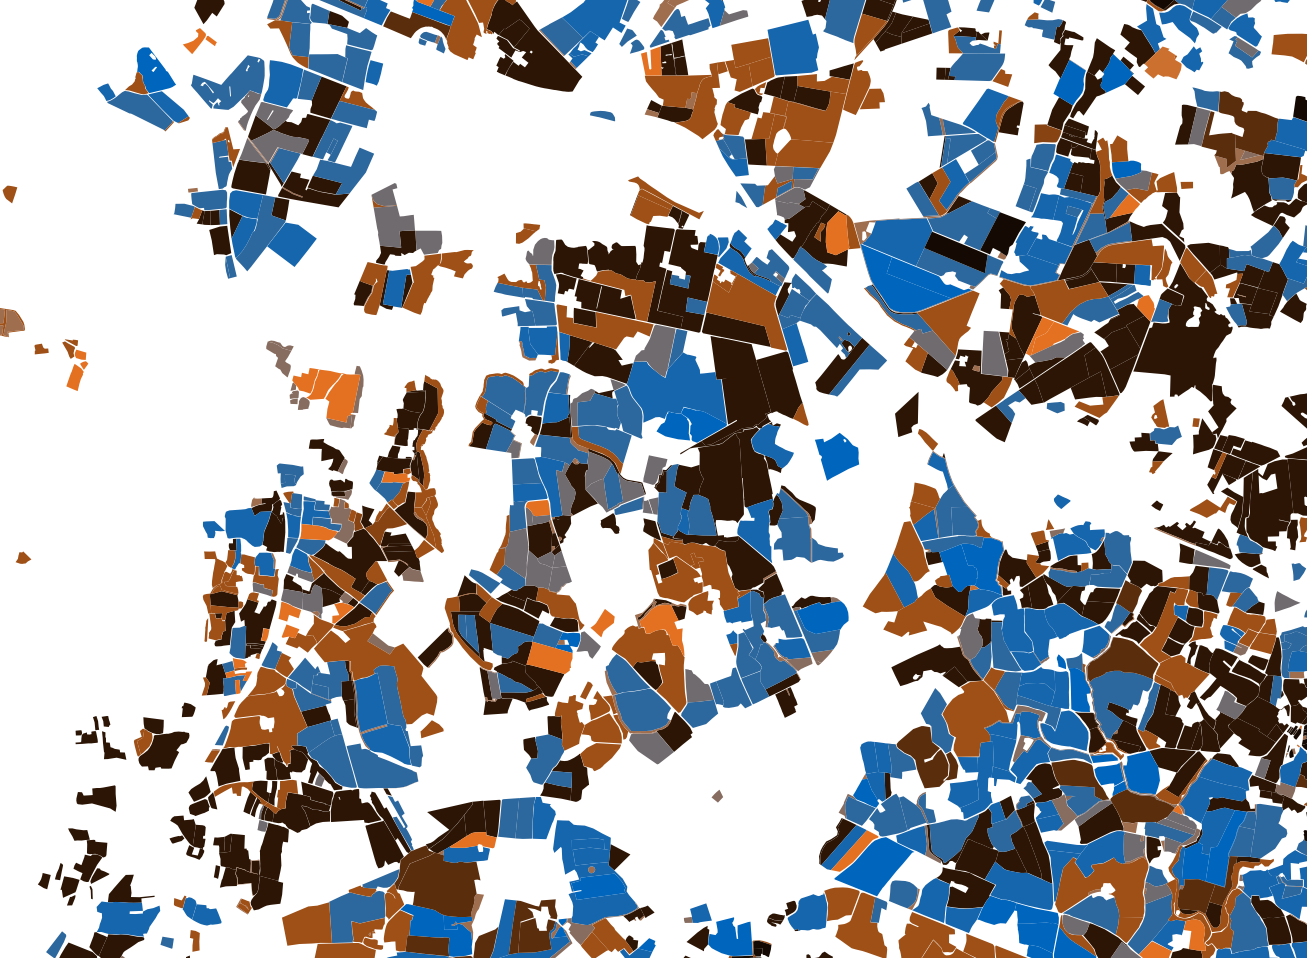
\includegraphics[width=15cm]{images/map/parcels}};
%	
%	
%	
%	\draw (x) -- (f) -- (y);
%	\end{tikzpicture}
\end{minipage}

\vspace{10em}
%
%\begin{tikzpicture}[node distance=4cm]
%
%	\node[draw](satellitedata){\satellitebox};
%	\node[draw, right=of satellitedata](model){\modelbox};
%	\node[draw, right=of model](label){\labelbox};
%	
%	\draw[-{stealth[scale=100]}] (satellitedata) -- (model);
%	\draw[-stealth] (model) -- (label);
%	
%\end{tikzpicture}

\section{The Dataset}

\begin{tikzpicture}[scale=5]
	\node(breizh){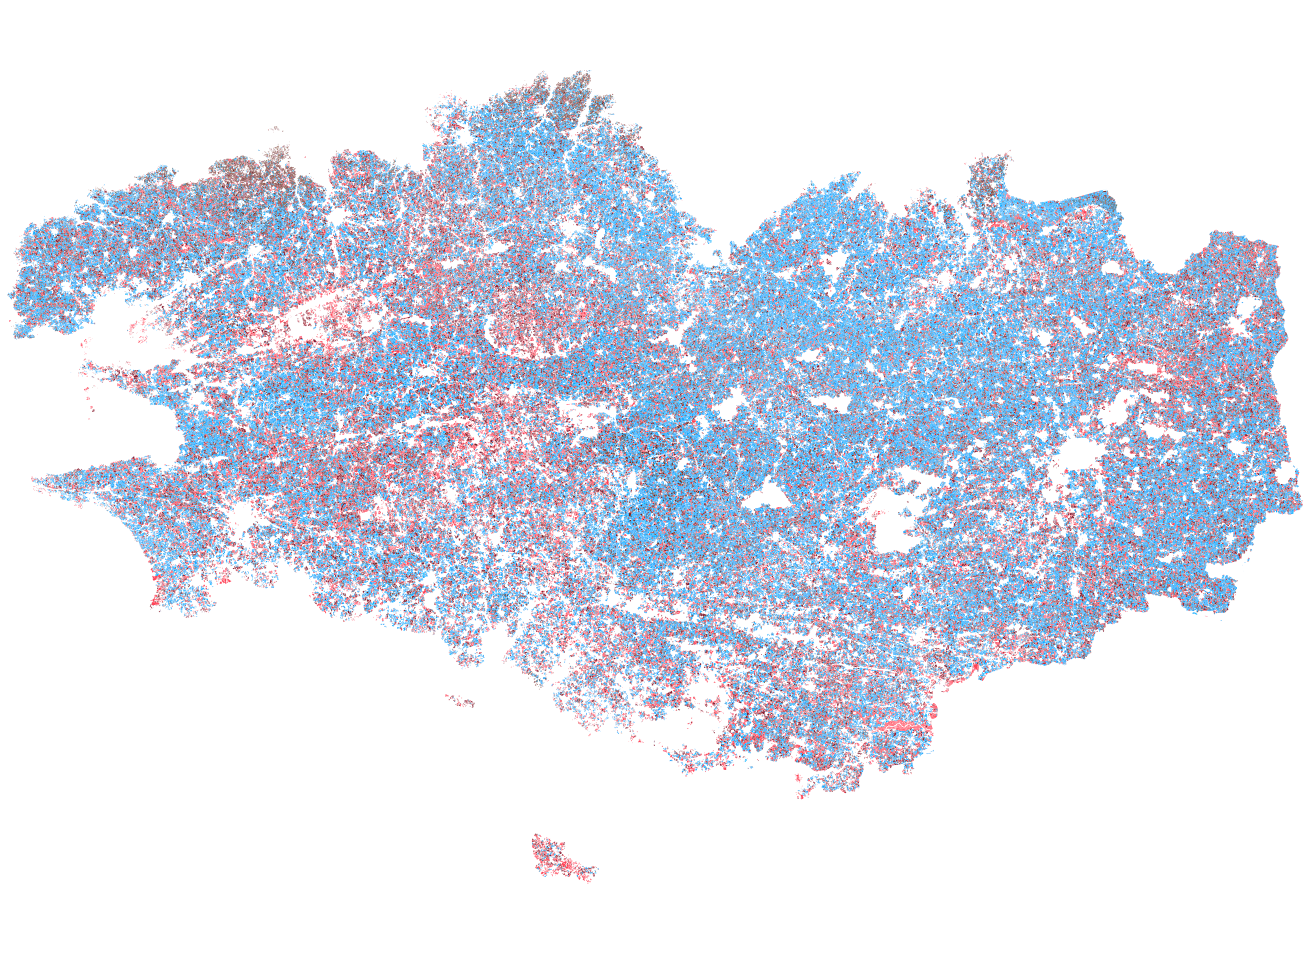
\includegraphics[width=30cm]{images/map/breizh}};
	\node at (1,-1){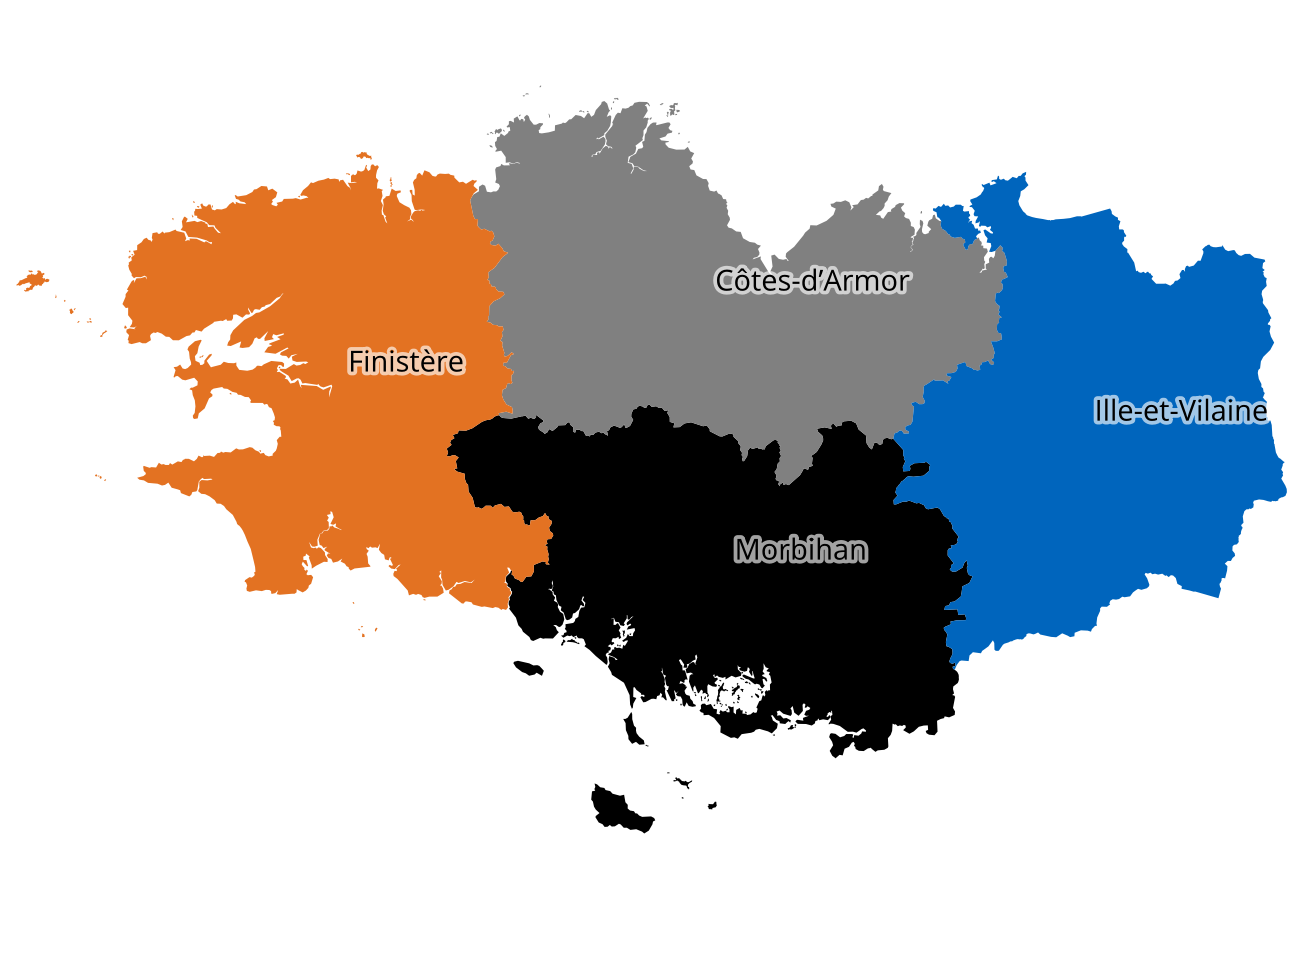
\includegraphics[width=10cm]{images/map/regions}};
	\node(europe) at (2,-2){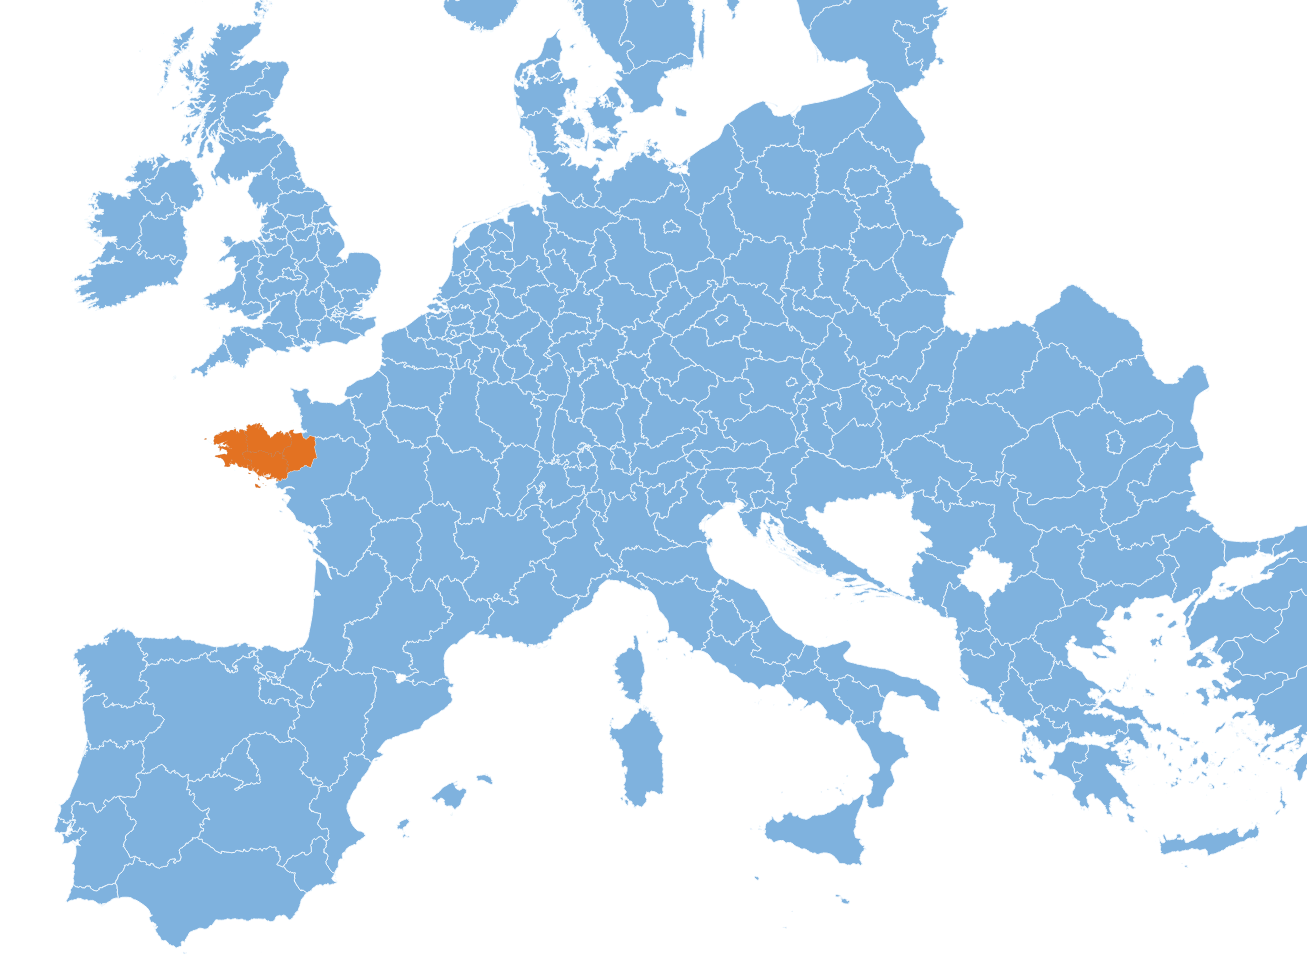
\includegraphics[width=10cm]{images/map/europe}};
	
\end{tikzpicture}



\vspace{30cm}

\vfill
\begin{tikzpicture}[scale=20]
	
		

	
%	\node at (1,0){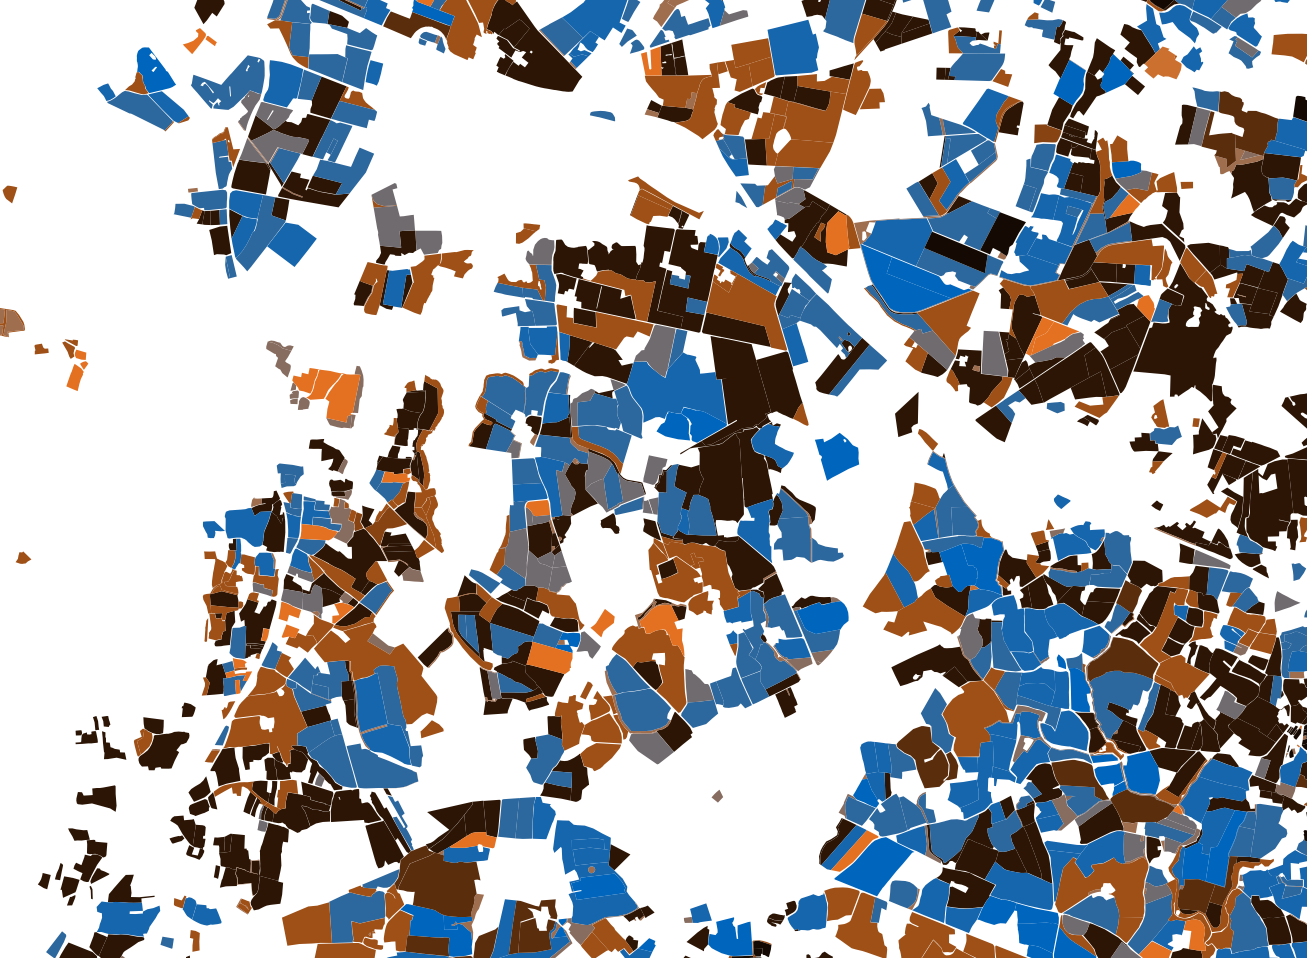
\includegraphics[width=10cm]{images/map/parcels}};
%	\node(breizh){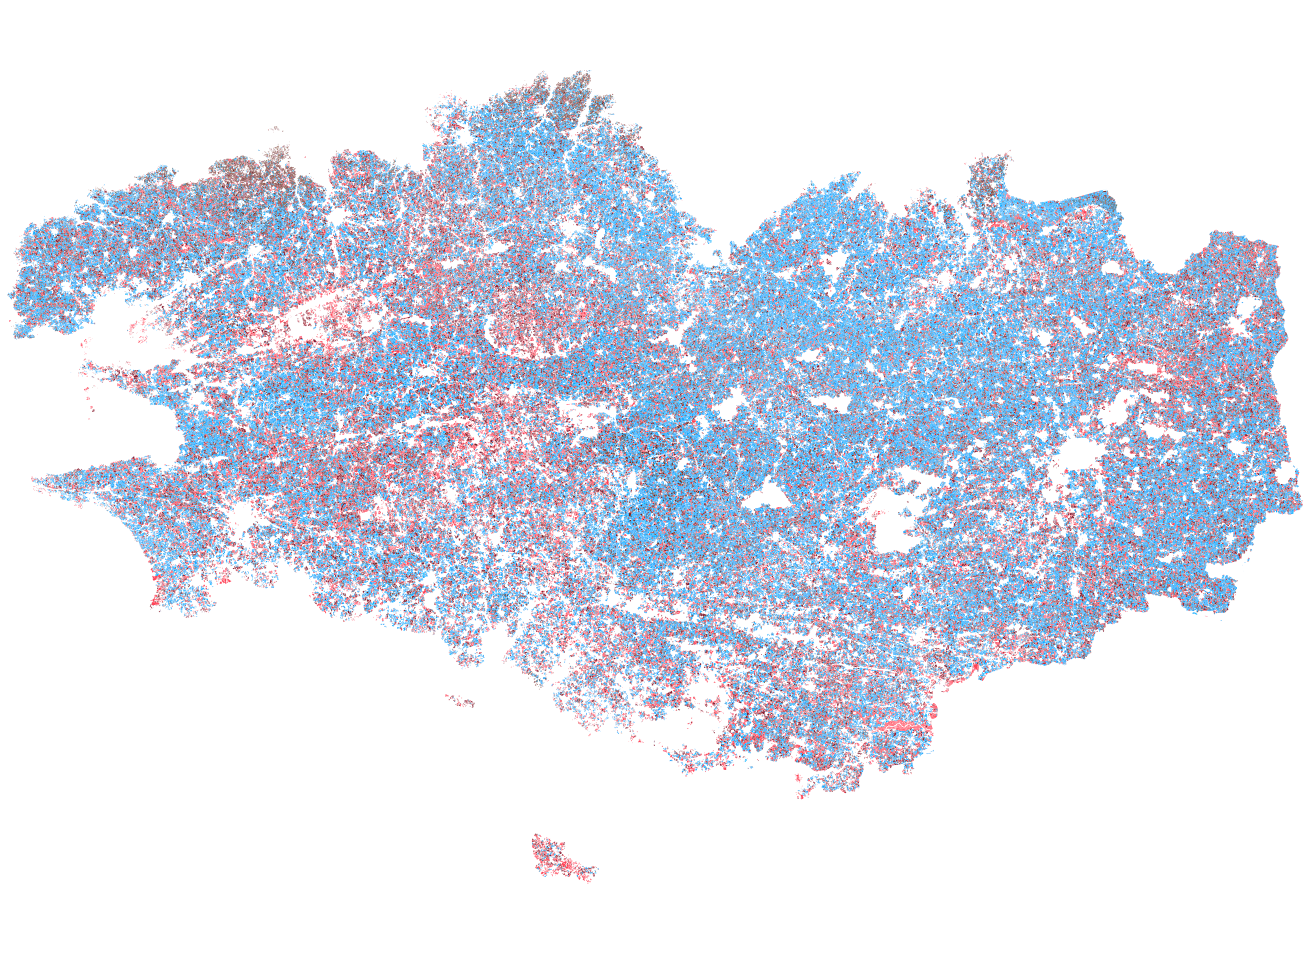
\includegraphics[width=10cm]{images/map/breizh}};
%	\node[below left =of breizh]{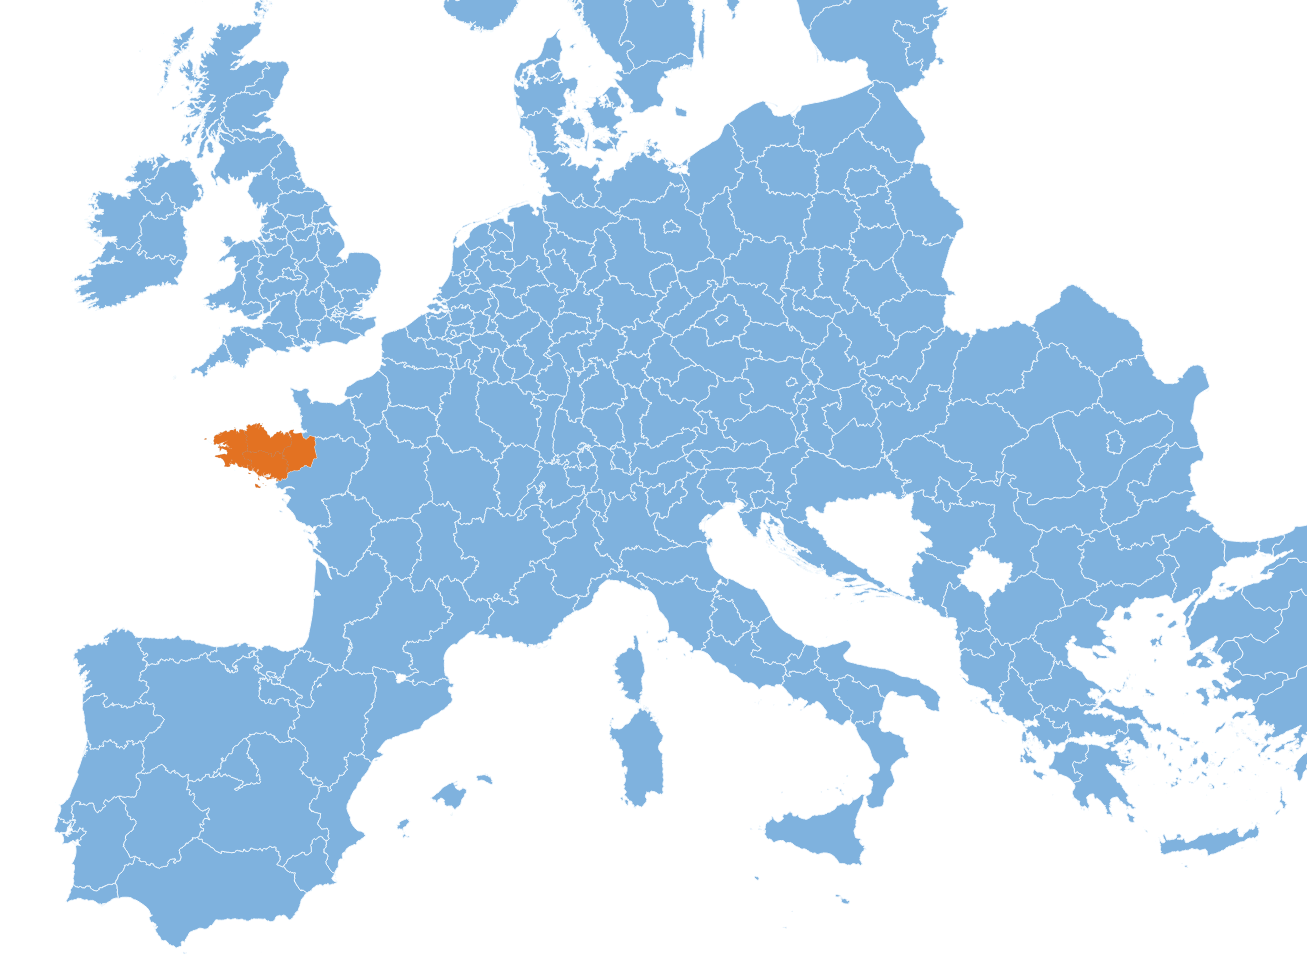
\includegraphics[width=10cm]{images/map/europe}};
%	\node[below right =of breizh]{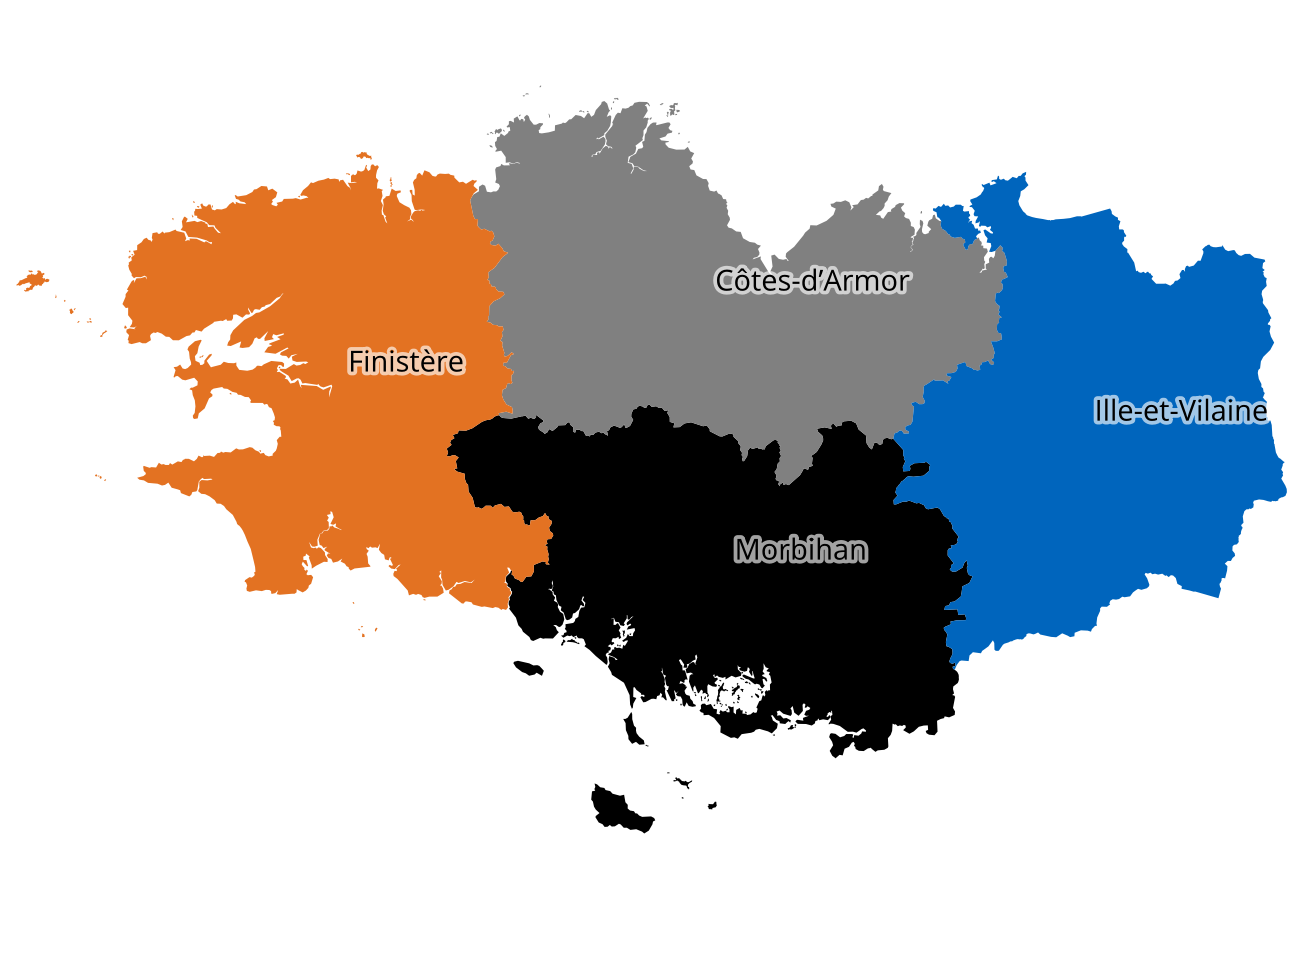
\includegraphics[width=10cm]{images/map/regions}};
	
	\node at (1,1){
		\begin{tabular}{lrr}
		\toprule
		Departements & NUTS-3 & Parcels \\
		\cmidrule(lr){1-1}\cmidrule(lr){2-2}\cmidrule(lr){3-3}
		%			\midrule
		Morbihan & FRH04 & 158522 \\
		Côtes-d’Armor & FRH01 & 221095 \\
		Finistère & FRH02 & 180565\\
		Ille-et-Vilaine & FRH03 & 207993\\
		\bottomrule
		\end{tabular}
	};



\node at (2,1){
	\confmat{images/data/BreizhCrops_rnn/npy/confmat_flat.csv}{3}{1}
};

\node at (2,2){
\begin{tabular}{rlcccc}
\toprule
\textbf{\#} & \textbf{crop type} &  \textbf{prec.} & \textbf{rec.} & \textbf{$f_1$} & \textbf{\#samples} \\
\cmidrule(lr){1-1}\cmidrule(lr){2-2}\cmidrule(lr){3-3}\cmidrule(lr){4-4}\cmidrule(lr){5-5}\cmidrule(lr){6-6}
%\midrule
1 & barley &         90 &          86 &          88 &     4982 \\
2 & wheat &         83 &          95 &          89 &    13850 \\
3 & corn &         93 &          \textbf{96} &          94 &    25059 \\
4 & fodder &         51 &          34 &          41 &     3449 \\
5 & fallow &         30 &           2 &           4 &     3863 \\
6 & misc. &         50 &          49 &          49 &    12499 \\
7 & orchards &         21 &           7 &          10 &      391 \\
8 & cereals &         74 &          47 &          57 &     4645 \\
9 & perm. meadows &         51 &          47 &          49 &    20966 \\
10 & protein crops &         42 &          61 &          50 &      498 \\
11 & rapeseed &         \textbf{96} &          94 &          \textbf{95} &     2664 \\
12 & temp. meadows &         56 &          68 &          62 &    29977 \\
13 & vegetables &         86 &          69 &          76 &     3114 \\
   &                       &            &             &             &          \\
   &                       &         \textbf{63} &          \textbf{58} &          \textbf{59} &   125957 \\
\bottomrule
\end{tabular}


};

\node at (2,0){
\begin{tabular}{lrrrrrrr}
\toprule
baseline & accuracy & $\kappa$ & mean f1 & mean precision  & mean recall \\
\cmidrule(lr){1-1}\cmidrule(lr){2-2}\cmidrule(lr){3-3}\cmidrule(lr){4-4}\cmidrule(lr){5-5}\cmidrule(lr){6-6}\cmidrule(lr){7-7}
Transformer & \textbf{0.69}  &  \textbf{0.63} & 0.57 & {0.60} & 0.56 \\
LSTM & 0.68 & 0.62 & \textbf{0.59} & \textbf{0.63} & \textbf{0.58} \\
\bottomrule
\end{tabular}
};
	
\node[text width=20cm] at (3,0){
Challenges
\begin{itemize}
	\item Imbalanced class labels
	\item Classes with similar characteristics
	\item Non-Gaussian noise induced by clouds
	\item Regional variations in the class distributions
	\item Irregular sampling distance
	\item Variable sequence length
	\item Spatial autocorrelation
\end{itemize}
};

	
\end{tikzpicture}

\hfill

% footer environment places \hfill and sets fontsize
\begin{footer}
	\begin{multicols}{2}
		\textbf{Technical University of Munich}\\
		TUM Department of Civil, Geo and Environmental Engineering \\
		Remote Sensing Technology, Computer Vision Research Group \\
		Arcisstr. 21, 80333 Munich, Germany \\
		www.lmf.bgu.tum.de/vision
	\vfill\columnbreak
	%right
		\textbf{Authors} \\
		Marc Rußwurm \\ (marc.russwurm@tum.de) \\
		Sébastien Lefèvre \\
		Marco Körner \\ (marco.koerner@tum.de)
	\vfill
	\end{multicols}
\end{footer}

\end{document}